\documentclass[11pt,a4paper]{article}
%% GENERATED FILE — do not hand-edit.
%% Rebuild: yarn build:advanced-manual
%% (narration lives in packages/subspace-lattice-react/src/tutorial/)

\usepackage[margin=0.8in]{geometry}
\usepackage{graphicx}
\usepackage{enumitem}
\usepackage{xcolor}
\usepackage{hyperref}

\graphicspath{{./}}

%% One annotated ply: diagram, move heading, coaching text.
\newcommand{\plyfig}[3]{%
  \begin{minipage}[t]{0.47\textwidth}
    \centering
    \includegraphics[width=0.94\linewidth]{#1}\\[0.3em]
    \begin{minipage}{0.96\linewidth}
      {\small\textbf{#2}}\\[0.15em]
      {\footnotesize #3}
    \end{minipage}
  \end{minipage}}

\hypersetup{colorlinks=true, linkcolor=black, urlcolor=blue!50!black}

\title{Subspace Lattice\\[0.4em]\large The Advanced Manual\\
\normalsize Three fully annotated games from the Fleet Academy}
\author{Interstellar Warp Gaming Federation \\ Digital Defiance}
\date{Rules version \texttt{hybrid-fleet} \\ Companion to the Official Rules (\texttt{rules.pdf})}

\begin{document}
\maketitle

\begin{abstract}
\noindent
This manual replays the guided Fleet Academy missions with every ply
diagrammed and explained: a short Surgical Strike highlight reel, a full
57-ply battle, a \texttt{hybrid-fleet} siege decided by the sector clock, and
Mission 4 --- Lockout via Command Overload (EMP). Part I teaches how to think
--- fleet geometry including optional Refractors and Carriers, reading
positions, valuing moves, and looking ahead. Later parts walk the games. Each
diagram shows the position \emph{after} the numbered ply; the moved ship's
squares glow.
\end{abstract}

\tableofcontents
\clearpage

\part{How to think in Subspace Lattice}

\section{Fleet geometry: three sliding profiles}

Rated online play still opens with twin Beams (Standard Beams). Advanced lobby
modules can authorize \textbf{Refractor Wing} or \textbf{Fleet Draft} --- same
Sensor Net law, wider geometry. Learn all three heavy profiles as one system so
orthogonal blockades never feel like a complete shield.

\begin{description}
  \item[The Orthogonal Lane (Beams)] Rook-equivalent slides, restricted
        entirely to your active Sensor Net. The shipping default wing line.
  \item[The Diagonal Vector (Refractors)] Bishop-equivalent slides under the
        same net law. Refractors map across the corners of Chebyshev radiation
        boundaries and exploit blind spots left by pure orthogonal setups ---
        especially the diagonals that brush the Anomalous Core at $(5,5)$.
  \item[The Omni-Directional Anchor (Carriers)] Queen-equivalent slides while
        Hub-anchored (Chebyshev distance $\le$ Hub sensor radius, $3$ under
        fleet defaults). Drift outside that tether and the Carrier crawls one
        king-step (or one orthogonal step if Target Locked). Dual nature from
        the first page: fortress at home, rubber band if it overextends.
\end{description}

Target Lock still reduces Refractor and Carrier to a single orthogonal step.
No active net, no heavy slide --- for any of the three.

\section{How to read a position}

Every diagram in this manual shows four things at once. Learn to scan them in
this order:

\begin{enumerate}
  \item \textbf{Hub safety.} Where is each Command Hub, and can anything reach
        it \emph{next ply}? This question outranks every other. Most decided
        fleet games end by Surgical Strike, and most Surgical Strikes are
        walk-ins that the loser could have seen one move earlier. Check
        orthogonal \emph{and} diagonal approach lanes.
  \item \textbf{The nets.} Blue is White's Sensor Net, red is Black's, purple
        overlap is Contested Space (it counts for neither side's sector
        coverage). The net is not decoration: Beams, Refractors, and Carriers
        may only execute multi-square slides inside their own glow, and an
        enemy standing in your net is Target Locked.
  \item \textbf{Locked ships.} A Target Locked ship moves one orthogonal step,
        nothing else. A locked Beam or Refractor is a wall ornament; a locked
        Carrier cannot slide; a locked Infiltrator cannot warp. Count locked
        ships before you count material.
  \item \textbf{Link integrity.} Escorts only radiate while chained to the Hub
        (friendly ships no more than two squares apart). One careless step can
        silently unplug half your net.
\end{enumerate}

\section{What a move is worth}

Chess players value material; Go players value territory. Lattice asks you to
price three currencies at once:

\begin{description}
  \item[Material] Captures matter, but a dead Escort that was not radiating is
        worth less than one holding your net together. Heavy pieces sit higher
        on the ladder (below).
  \item[Coverage] Net cells are mobility for your heavy slides, Target Locks
        against the enemy, and --- after the sector clock arms --- a win
        condition. Diagonal coverage from a Refractor is real territory even
        when no orthogonal file is open.
  \item[Tempo] White moves first and holds the Initiative Relay Escort as
        compensation for having to commit first. Spending a ply on a move that
        neither threatens nor builds hands the initiative back. A Carrier that
        must crawl home after drifting has spent tempo twice.
\end{description}

\paragraph{Heavy-piece hierarchy (when the wing is in play).}
\begin{itemize}
  \item \textbf{Refractor --- high coverage, specialized material.} It commands
        massive diagonal reach across Chebyshev radiation squares but cannot
        hold a purely orthogonal line. Trading Beam for Refractor is usually
        lateral; trading an Escort for a Refractor is a massive tactical win.
  \item \textbf{Carrier --- maximum material, conditional tempo.} The ultimate
        defensive juggernaut while tethered: omni-directional slide dominates
        Material and Coverage, but pushing it up the board sacrifices Tempo
        when the Hub-anchor snaps. Prefer locking the home rank with the
        Carrier so Beams and Refractors can press; do not treat an untethered
        Carrier as a queen.
\end{itemize}

The recurring beginner error is over-valuing material: trading an active
linked Escort for a passive one is usually a loss even though the count says
even.

\section{Thinking ahead: the look-ahead scan}

Before every move, in order:

\begin{enumerate}
  \item \textbf{Can I take their Hub?} If yes, play it. The game ends. Scan
        Beam files \emph{and} Refractor diagonals (including slices past the
        Anomaly corners).
  \item \textbf{Can they take mine after my intended move?} Simulate your
        candidate, then check every enemy reply against your Hub square.
        If any reply lands there, your Hub is \emph{hanging} --- one ply from
        Surgical Strike. The rules still allow that move; the discipline is
        not to play it. Find another candidate. The academy drills this as
        \emph{refuse the hang}: never leave the flagship where they can
        capture it next. Orthogonal screens do not answer diagonal threats.
  \item \textbf{What does the move do for the nets?} Prefer moves that answer
        two ways at once: extend coverage \emph{and} threaten, retreat
        \emph{and} keep the chain linked.
  \item \textbf{Are my corners exposed to a Refractor slice?} The Anomalous
        Core at $(5,5)$ blocks orthogonal Beam paths through its row and
        column, so players feel safe behind that screen. Explicitly scan the
        diagonal vectors that brush the Anomaly's corners --- Refractors
        bypass orthogonal walls that look airtight.
  \item \textbf{Is the enemy Carrier tethered or drifting?} Instantly price
        Chebyshev distance from Carrier to its Command Hub. Within radius $3$
        (fleet defaults), treat it as an omni-directional lethal threat.
        Outside that radius, downgrade it to a single-step piece until it
        re-enters the Hub's radiation.
\end{enumerate}

Depth beyond one reply comes from asking question 2 recursively about forcing
lines only: captures, Hub threats, and moves that lock a key enemy ship.
Quiet positions do not need deep trees; sharp ones do.

\section{Openings: the first ten plies}

The mirrored fleet plus White's relay Escort makes openings about
\emph{structure}, not gambits:

\begin{itemize}
  \item Advance central Escorts first --- they carry the net forward and screen
        the Hub file.
  \item Keep every Escort within two squares of the chain. A linked fleet
        walks; an unlinked one crawls.
  \item Beams want \emph{prepared} files: slide them early inside your net to
        a lane that will point at the enemy Hub once coverage arrives.
  \item Under Refractor Wing or Fleet Draft, park heavies on files $3$ and $7$
        already inside the opening net. A Refractor contest of the center works
        differently than a Beam file claim --- diagonals matter from ply one.
  \item Under Fleet Draft, treat the Carrier as a home-rank fortress. Its
        Hub-anchor is a natural rubber band: early aggression that drifts it
        off the Hub trades capital mobility for a crawl.
  \item The Gravity Well at (5,5) splits the board. Decide early which side of
        it your pressure will live on --- and which diagonal seams you will
        contest around its corners.
\end{itemize}

\section{Midgame: pressure without overextension}

Mission 2 (Standard Beams) is the orthogonal model: net pressure, Target Lock
threats, and probing for a Hub mistake --- not racing to paint the map.
Overextended ships end up inside the enemy glow, locked, and become targets.
Watch for the moment an enemy Beam's lane \emph{or} Refractor diagonal and
your Hub share a clear path: that is when defensive plies stop being optional.
When a Carrier is on the board, re-check tether status every few plies --- the
same ship flips from fortress to foot soldier when it drifts.

\section{Pedagogical highlight: the Anomaly Slice}

Missions 1--3 below stay on Standard Beams so the rated opening stays
readable. This midgame sketch teaches the Refractor's job when Heavy wings
are authorized --- call it \emph{the 45-ply blind spot}.

\begin{description}
  \item[Setup] White has built a strong orthogonal blockade with Beams along
        a midboard rank, screening the Hub. Black's Escorts cannot find a
        clean breach on the files.
  \item[Execution] Black maneuvers a Refractor into active Sensor Net on a
        diagonal that brushes a corner of the $(5,5)$ Anomaly.
  \item[Lesson] White's orthogonal wall is blind to that vector. The diagonal
        slide past the Anomaly bypasses the Beams entirely and can force a
        Target Lock on White's Hub --- or open a Surgical Strike lane the
        Beam screen never saw. Orthogonal safety is incomplete safety.
\end{description}

\section{Endgame: strike, clock, or Lockout}

Three finishes exist. If a Hub hunt is winning, convert like Mission 1 and 2:
clear the lane (file or diagonal), keep your Hub from hanging, strike. If both
fleets dig
in, the sector clock (armed at ply 100 under fleet rules) turns coverage into
the win condition --- Mission 3. Late game, every net cell is a point on the
scoreboard, Contested Space is a weapon (project into their net to stall
their streak), and passive defense finally loses on the clock instead of
drawing forever.

The third finish is \textbf{Lockout}: leave the opponent with zero legal
replies. Bodies alone almost never force that against a live Command Hub --- a
cornered Hub can still capture its way out. Under \texttt{hybrid-fleet},
\textbf{Command Overload (EMP)} is the practical path:

\begin{itemize}[leftmargin=*]
  \item Charge only while your Hub stays put: each non-Hub ply of yours adds
        one to EMP charge; moving the Hub (or firing) resets it to zero.
  \item Default charge target is $15$ non-Hub plies; blast radius is Chebyshev
        $3$ from the Hub (lobby-tunable).
  \item Firing EMP \emph{is} your entire turn. Enemy ships inside the radius
        cannot move or capture for \texttt{empBlackoutPlies} of \emph{their}
        replies (default $1$). Your own fleet is never in the blast --- the
        cost is the spent turn, not friendly fire.
  \item If every remaining enemy ship is seized, \texttt{listLegalMoves} is
        empty and you win with \texttt{winnerReason=no-moves}.
\end{itemize}

Expanded branching from Refractors and Carriers does not change the win
conditions --- it changes which geometries feed them.

\clearpage

\part{The annotated games}
\section{Mission 1 --- Surgical Strike, the highlight reel}
Guided mission 1 of 3. A short, fixed highlight reel---not a full match. Tap Play and watch each order. White grows the net, keeps the Hub from hanging (capturable next turn), then Surgical Strike. Black shows the usual counterplay and death-trap temptation.

\begin{center}

\includegraphics[width=0.55\textwidth]{figures/missions/mission-short-strike/ply-000}\\
{\small\textbf{Starting position.}}
\end{center}
\clearpage
\plyfig{figures/missions/mission-short-strike/ply-001}{Ply 1 --- White Escort (5,3)$\rightarrow$(5,4)}{White opens by pushing the Initiative Relay Escort. Going first already has a forward foothold; deepening it grows midboard coverage so later Beam fire has somewhere to live.\; {\color{gray}\scriptsize [net 34--42 \,\textbullet\, 4 ships locked]}}%
\hfill
\plyfig{figures/missions/mission-short-strike/ply-002}{Ply 2 --- Black Escort (8,8)$\rightarrow$(8,7)}{Black does not yet contest the Beam's file. A quiet side step keeps options open while White telegraphs net-building on the left.\; {\color{gray}\scriptsize [net 34--42 \,\textbullet\, 4 ships locked]}}%

\vspace{0.9em}

\plyfig{figures/missions/mission-short-strike/ply-003}{Ply 3 --- White Escort (3,2)$\rightarrow$(3,3)}{White's Beam is still boxed inside a small net. Sliding an Escort beside the file extends the blue glow toward Black's Hub without sitting on the lane (which would block the shot).\; {\color{gray}\scriptsize [net 36--42 \,\textbullet\, 5 ships locked]}}%
\hfill
\plyfig{figures/missions/mission-short-strike/ply-004}{Ply 4 --- Black Escort (6,1)$\rightarrow$(5,1)}{Black reaches for a classic beginner trap: step next to White's Hub. If White greedily stares at the Beam shot and ignores this, Black takes Surgical Strike next.\; {\color{gray}\scriptsize [net 36--42 \,\textbullet\, 5 ships locked \,\textbullet\, \textbf{Hub en prise!}]}}%

\vspace{0.9em}

\clearpage
\plyfig{figures/missions/mission-short-strike/ply-005}{Ply 5 --- White Escort (4,1)$\rightarrow$(5,1)}{White's Hub was hanging --- Black could capture it next turn and win. Refuse the hang: take the threatening Escort now. The prepared Beam shot can wait one ply.\; {\color{gray}\scriptsize [captures Escort \,\textbullet\, net 36--42 \,\textbullet\, 4 ships locked]}}%
\hfill
\plyfig{figures/missions/mission-short-strike/ply-006}{Ply 6 --- Black Escort (8,7)$\rightarrow$(8,6)}{Black's tactical shot failed. With no immediate recapture, Black shuffles---tempo lost, Hub still sitting on White's Beam file.\; {\color{gray}\scriptsize [net 36--42 \,\textbullet\, 4 ships locked \,\textbullet\, \textbf{Hub en prise!}]}}%

\vspace{0.9em}

\plyfig{figures/missions/mission-short-strike/ply-007}{Ply 7 --- White Beam (2,0)$\rightarrow$(2,4)}{Net open, Hub safe, enemy Hub on the Beam's file. White converts preparation into Surgical Strike---the usual way fleet games end when the plan works.\; {\color{gray}\scriptsize [captures Command Hub \,\textbullet\, net 36--0 \,\textbullet\, \textbf{White wins}]}}%

\vspace{0.9em}


\vspace{1em}
\noindent\textbf{Debrief.} Mission complete. White wins by Surgical Strike. Next: a chess-length battle (\textasciitilde{}50 plies), then a clock finish when Hubs survive.
\clearpage
\section{Mission 2 --- A standard battle (57 plies)}
Guided mission 2 of 3. Fixed 57-ply game: White is building toward Surgical Strike --- park Beams, grow Escorts so those Beams can ride, march the Hub for coverage, then peel the enemy Hub's screen. Quiet hops are just relay work; use ``Play next 5'' to skim them.

\begin{center}

\includegraphics[width=0.55\textwidth]{figures/missions/mission-standard-battle/ply-000}\\
{\small\textbf{Starting position.}}
\end{center}
\clearpage
\plyfig{figures/missions/mission-standard-battle/ply-001}{Ply 1 --- White Beam (2,0)$\rightarrow$(2,3)}{White climbs the left Beam off the back rank. Beams cannot invent a path --- they only slide inside Sensor Net --- so parking now means the dreadnought is already on a file when Escorts later grow the glow toward Black.\; {\color{gray}\scriptsize [net 31--28]}}%
\hfill
\plyfig{figures/missions/mission-standard-battle/ply-002}{Ply 2 --- Black Beam (2,10)$\rightarrow$(2,7)}{Black mirrors on the opposite wing. Same logic: get the long-range piece onto a file before the Escorts start laying relays.\; {\color{gray}\scriptsize [net 31--28]}}%

\vspace{0.9em}

\plyfig{figures/missions/mission-standard-battle/ply-003}{Ply 3 --- White Beam (8,0)$\rightarrow$(8,3)}{White's second Beam leaves the corner. Corner Beams are stranded until coverage arrives; mid-file parking is cheaper tempo once the relay chain starts.\; {\color{gray}\scriptsize [net 31--28]}}%
\hfill
\plyfig{figures/missions/mission-standard-battle/ply-004}{Ply 4 --- Black Beam (2,7)$\rightarrow$(5,7)}{Black swings onto column 5 --- the file Black's own Hub sits on, and the one White will eventually need to contest. Central Beams matter once anyone's net reaches midboard.\; {\color{gray}\scriptsize [net 31--28]}}%

\vspace{0.9em}

\clearpage
\plyfig{figures/missions/mission-standard-battle/ply-005}{Ply 5 --- White Beam (8,3)$\rightarrow$(6,3)}{White tucks onto column 6 beside the Hub file. Two Beams flanking the center means whichever Escort chain grows first already has a rider waiting.\; {\color{gray}\scriptsize [net 31--28]}}%
\hfill
\plyfig{figures/missions/mission-standard-battle/ply-006}{Ply 6 --- Black Beam (8,10)$\rightarrow$(8,7)}{Black Beam to (8,7).\; {\color{gray}\scriptsize [net 31--28]}}%

\vspace{0.9em}

\plyfig{figures/missions/mission-standard-battle/ply-007}{Ply 7 --- White Beam (2,3)$\rightarrow$(4,3)}{Left Beam steps to column 4. White now owns the two files most likely to become Hub-hunt lanes once coverage stretches forward --- not attacking yet, just choosing where the shot will come from.\; {\color{gray}\scriptsize [net 31--28]}}%
\hfill
\plyfig{figures/missions/mission-standard-battle/ply-008}{Ply 8 --- Black Beam (8,7)$\rightarrow$(6,7)}{Black's last Beam joins column 6. Opening placement is done; the next job belongs to Escorts, who actually grow the nets those Beams will ride.\; {\color{gray}\scriptsize [net 31--28]}}%

\vspace{0.9em}

\clearpage
\plyfig{figures/missions/mission-standard-battle/ply-009}{Ply 9 --- White Escort (4,0)$\rightarrow$(4,1)}{First Escort hop. Escorts are the only ships that push Sensor Net into unmapped dark --- without this chain, the parked Beams stay boxed in their starting glow.\; {\color{gray}\scriptsize [net 31--28]}}%
\hfill
\plyfig{figures/missions/mission-standard-battle/ply-010}{Ply 10 --- Black Escort (5,9)$\rightarrow$(5,8)}{Black Escort to (5,8).\; {\color{gray}\scriptsize [net 31--28]}}%

\vspace{0.9em}

\plyfig{figures/missions/mission-standard-battle/ply-011}{Ply 11 --- White Escort (6,0)$\rightarrow$(6,1)}{White Escort to (6,1).\; {\color{gray}\scriptsize [net 31--28]}}%
\hfill
\plyfig{figures/missions/mission-standard-battle/ply-012}{Ply 12 --- Black Command Hub (5,10)$\rightarrow$(5,9)}{Black's Hub edges forward. The Hub is the net's power anchor, so this is not king-walking for its own sake --- red coverage jumps because the whole lattice moves with the flagship.\; {\color{gray}\scriptsize [net 31--35]}}%

\vspace{0.9em}

\clearpage
\plyfig{figures/missions/mission-standard-battle/ply-013}{Ply 13 --- White Escort (5,3)$\rightarrow$(5,4)}{White's forward Escort (the first-mover's extra relay) steps to (5,4). That is the point of the Relay: early midboard coverage so White's Beams get lanes before Black can match.\; {\color{gray}\scriptsize [net 34--35]}}%
\hfill
\plyfig{figures/missions/mission-standard-battle/ply-014}{Ply 14 --- Black Escort (6,10)$\rightarrow$(5,10)}{Black Escort to (5,10).\; {\color{gray}\scriptsize [net 34--35]}}%

\vspace{0.9em}

\plyfig{figures/missions/mission-standard-battle/ply-015}{Ply 15 --- White Beam (6,3)$\rightarrow$(6,5)}{White's Beam slides to (6,5) because the Escort chain finally covers the path. The advance is the payoff for plies 9--13 --- Beams only move when the net lets them.\; {\color{gray}\scriptsize [net 34--35]}}%
\hfill
\plyfig{figures/missions/mission-standard-battle/ply-016}{Ply 16 --- Black Beam (5,7)$\rightarrow$(5,6)}{Black answers on (5,6). Midboard Beams are there to punish an overextended Escort or to sit on a file the enemy Hub might wander onto.\; {\color{gray}\scriptsize [net 34--35]}}%

\vspace{0.9em}

\clearpage
\plyfig{figures/missions/mission-standard-battle/ply-017}{Ply 17 --- White Beam (4,3)$\rightarrow$(4,5)}{White's column-4 Beam reaches (4,5). Coverage dips briefly because the piece left a square the net was using; the bet is Escorts will re-link before Black can exploit the hole.\; {\color{gray}\scriptsize [net 28--35]}}%
\hfill
\plyfig{figures/missions/mission-standard-battle/ply-018}{Ply 18 --- Black Beam (6,7)$\rightarrow$(5,7)}{Black Beam to (5,7).\; {\color{gray}\scriptsize [net 28--35]}}%

\vspace{0.9em}

\plyfig{figures/missions/mission-standard-battle/ply-019}{Ply 19 --- White Escort (4,1)$\rightarrow$(4,2)}{Escort to (4,2) snaps blue coverage back. This is the usual repair job after a Beam advance: reconnect the daisy-chain so the forward dreadnought stays fed.\; {\color{gray}\scriptsize [net 34--35]}}%
\hfill
\plyfig{figures/missions/mission-standard-battle/ply-020}{Ply 20 --- Black Escort (4,10)$\rightarrow$(4,9)}{Black Escort to (4,9).\; {\color{gray}\scriptsize [net 34--35]}}%

\vspace{0.9em}

\clearpage
\plyfig{figures/missions/mission-standard-battle/ply-021}{Ply 21 --- White Escort (4,2)$\rightarrow$(5,2)}{White Escort to (5,2).\; {\color{gray}\scriptsize [net 34--35]}}%
\hfill
\plyfig{figures/missions/mission-standard-battle/ply-022}{Ply 22 --- Black Escort (4,9)$\rightarrow$(4,8)}{Black Escort to (4,8).\; {\color{gray}\scriptsize [net 34--35]}}%

\vspace{0.9em}

\plyfig{figures/missions/mission-standard-battle/ply-023}{Ply 23 --- White Escort (5,2)$\rightarrow$(5,3)}{White Escort to (5,3).\; {\color{gray}\scriptsize [net 34--35]}}%
\hfill
\plyfig{figures/missions/mission-standard-battle/ply-024}{Ply 24 --- Black Escort (4,8)$\rightarrow$(4,7)}{Black Escort to (4,7).\; {\color{gray}\scriptsize [net 34--35]}}%

\vspace{0.9em}

\clearpage
\plyfig{figures/missions/mission-standard-battle/ply-025}{Ply 25 --- White Escort (5,1)$\rightarrow$(5,2)}{White Escort to (5,2).\; {\color{gray}\scriptsize [net 34--35]}}%
\hfill
\plyfig{figures/missions/mission-standard-battle/ply-026}{Ply 26 --- Black Escort (4,7)$\rightarrow$(4,6)}{Escort to (4,6) puts a White ship under Target Lock. Locks are the midgame punishment for standing in enemy glow --- a locked Beam crawls one step and stops being a long-range threat.\; {\color{gray}\scriptsize [net 34--38 \,\textbullet\, 1 ship locked]}}%

\vspace{0.9em}

\plyfig{figures/missions/mission-standard-battle/ply-027}{Ply 27 --- White Beam (4,5)$\rightarrow$(4,6)}{White's Beam takes that Escort. Removing the tip both lifts the lock and clears a square on the file White wants open for the Hub hunt.\; {\color{gray}\scriptsize [captures Escort \,\textbullet\, net 34--35 \,\textbullet\, 1 ship locked]}}%
\hfill
\plyfig{figures/missions/mission-standard-battle/ply-028}{Ply 28 --- Black Beam (5,6)$\rightarrow$(4,6)}{Black Beam recaptures. Trading a Beam for an Escort is often fine for White --- Escorts carry net, Beams only ride it --- but Black at least clears the immediate taker.\; {\color{gray}\scriptsize [captures Beam \,\textbullet\, net 34--35]}}%

\vspace{0.9em}

\clearpage
\plyfig{figures/missions/mission-standard-battle/ply-029}{Ply 29 --- White Escort (6,1)$\rightarrow$(5,1)}{White Escort to (5,1).\; {\color{gray}\scriptsize [net 34--35]}}%
\hfill
\plyfig{figures/missions/mission-standard-battle/ply-030}{Ply 30 --- Black Beam (4,6)$\rightarrow$(5,6)}{Black Beam to (5,6).\; {\color{gray}\scriptsize [net 34--35]}}%

\vspace{0.9em}

\plyfig{figures/missions/mission-standard-battle/ply-031}{Ply 31 --- White Command Hub (5,0)$\rightarrow$(6,1)}{White Hub leaves the back rank. Flagship steps expand Sovereign Space for every linked Escort; blue coverage jumps because the power anchor moved, not because a random Escort painted a cell.\; {\color{gray}\scriptsize [net 38--35]}}%
\hfill
\plyfig{figures/missions/mission-standard-battle/ply-032}{Ply 32 --- Black Command Hub (5,9)$\rightarrow$(6,8)}{Black Hub to (6,8). Once both flagships are mobile, coverage races and Target Locks appear; the board is no longer two back-rank museums.\; {\color{gray}\scriptsize [net 38--42 \,\textbullet\, 1 ship locked]}}%

\vspace{0.9em}

\clearpage
\plyfig{figures/missions/mission-standard-battle/ply-033}{Ply 33 --- White Command Hub (6,1)$\rightarrow$(6,2)}{White Hub to (6,2). Nets sit even. The march is still about owning the center files so Escorts and Beams can force Black's Hub into a bad square later.\; {\color{gray}\scriptsize [net 42--42 \,\textbullet\, 1 ship locked]}}%
\hfill
\plyfig{figures/missions/mission-standard-battle/ply-034}{Ply 34 --- Black Escort (5,10)$\rightarrow$(5,9)}{Black Escort to (5,9).\; {\color{gray}\scriptsize [net 42--42 \,\textbullet\, 1 ship locked]}}%

\vspace{0.9em}

\plyfig{figures/missions/mission-standard-battle/ply-035}{Ply 35 --- White Command Hub (6,2)$\rightarrow$(6,3)}{Hub to (6,3): blue leaps to 49 cells and two ships lock. That spike is what turns setup into a Hub hunt --- White's lattice finally covers the files Black's Hub has to live on.\; {\color{gray}\scriptsize [net 49--42 \,\textbullet\, 2 ships locked]}}%
\hfill
\plyfig{figures/missions/mission-standard-battle/ply-036}{Ply 36 --- Black Escort (5,9)$\rightarrow$(6,9)}{Black Escort to (6,9).\; {\color{gray}\scriptsize [net 49--42 \,\textbullet\, 2 ships locked]}}%

\vspace{0.9em}

\clearpage
\plyfig{figures/missions/mission-standard-battle/ply-037}{Ply 37 --- White Escort (5,4)$\rightarrow$(6,4)}{Escort to (6,4). A forward Hub without a linked relay is a coverage mirage --- one capture unplugs half the glow. This Escort is insurance for the march.\; {\color{gray}\scriptsize [net 49--42 \,\textbullet\, 2 ships locked]}}%
\hfill
\plyfig{figures/missions/mission-standard-battle/ply-038}{Ply 38 --- Black Beam (5,7)$\rightarrow$(6,7)}{Black Beam to (6,7).\; {\color{gray}\scriptsize [net 49--42 \,\textbullet\, 2 ships locked]}}%

\vspace{0.9em}

\plyfig{figures/missions/mission-standard-battle/ply-039}{Ply 39 --- White Escort (5,3)$\rightarrow$(5,4)}{White Escort to (5,4).\; {\color{gray}\scriptsize [net 49--42 \,\textbullet\, 2 ships locked]}}%
\hfill
\plyfig{figures/missions/mission-standard-battle/ply-040}{Ply 40 --- Black Beam (6,7)$\rightarrow$(6,5)}{Capture on (6,5). With dreadnoughts trading, the fight shifts to who still has Escorts holding the chain --- those are what keep the Hub hunt (or the defense) alive.\; {\color{gray}\scriptsize [captures Beam \,\textbullet\, net 49--42 \,\textbullet\, 2 ships locked]}}%

\vspace{0.9em}

\clearpage
\plyfig{figures/missions/mission-standard-battle/ply-041}{Ply 41 --- White Escort (6,4)$\rightarrow$(6,5)}{White Escort takes back. The point is not the piece count --- it is keeping a friendly body on the file White's Hub is climbing so Black cannot plant there for free.\; {\color{gray}\scriptsize [captures Beam \,\textbullet\, net 49--42 \,\textbullet\, 2 ships locked]}}%
\hfill
\plyfig{figures/missions/mission-standard-battle/ply-042}{Ply 42 --- Black Escort (5,8)$\rightarrow$(5,7)}{Black Escort to (5,7).\; {\color{gray}\scriptsize [net 49--42 \,\textbullet\, 2 ships locked]}}%

\vspace{0.9em}

\plyfig{figures/missions/mission-standard-battle/ply-043}{Ply 43 --- White Escort (5,1)$\rightarrow$(6,1)}{White Escort to (6,1).\; {\color{gray}\scriptsize [net 49--42 \,\textbullet\, 2 ships locked]}}%
\hfill
\plyfig{figures/missions/mission-standard-battle/ply-044}{Ply 44 --- Black Escort (5,7)$\rightarrow$(6,7)}{Black Escort to (6,7).\; {\color{gray}\scriptsize [net 49--42 \,\textbullet\, 2 ships locked]}}%

\vspace{0.9em}

\clearpage
\plyfig{figures/missions/mission-standard-battle/ply-045}{Ply 45 --- White Escort (5,2)$\rightarrow$(5,3)}{White Escort to (5,3).\; {\color{gray}\scriptsize [net 49--42 \,\textbullet\, 2 ships locked]}}%
\hfill
\plyfig{figures/missions/mission-standard-battle/ply-046}{Ply 46 --- Black Beam (5,6)$\rightarrow$(6,6)}{Black Beam to (6,6).\; {\color{gray}\scriptsize [net 49--42 \,\textbullet\, 2 ships locked]}}%

\vspace{0.9em}

\plyfig{figures/missions/mission-standard-battle/ply-047}{Ply 47 --- White Escort (6,5)$\rightarrow$(6,6)}{Escort takes on (6,6). No Black dreadnought left hanging over the Hub file means White can press the Hub without a Beam shot answering from midboard.\; {\color{gray}\scriptsize [captures Beam \,\textbullet\, net 52--42 \,\textbullet\, 2 ships locked]}}%
\hfill
\plyfig{figures/missions/mission-standard-battle/ply-048}{Ply 48 --- Black Escort (6,7)$\rightarrow$(6,6)}{Recapture. Coverage dips, but Black's real problem is screen thickness around the Hub, not the trade itself.\; {\color{gray}\scriptsize [captures Escort \,\textbullet\, net 49--42 \,\textbullet\, 1 ship locked]}}%

\vspace{0.9em}

\clearpage
\plyfig{figures/missions/mission-standard-battle/ply-049}{Ply 49 --- White Escort (5,4)$\rightarrow$(6,4)}{White Escort to (6,4).\; {\color{gray}\scriptsize [net 49--42 \,\textbullet\, 1 ship locked]}}%
\hfill
\plyfig{figures/missions/mission-standard-battle/ply-050}{Ply 50 --- Black Command Hub (6,8)$\rightarrow$(6,7)}{Hub to (6,7). Equal nets, but every step toward White's Escorts makes Surgical Strike one mistake away. Bold when you need coverage; fatal if the screen is thin.\; {\color{gray}\scriptsize [net 49--49 \,\textbullet\, 2 ships locked]}}%

\vspace{0.9em}

\plyfig{figures/missions/mission-standard-battle/ply-051}{Ply 51 --- White Escort (5,3)$\rightarrow$(5,4)}{White Escort to (5,4).\; {\color{gray}\scriptsize [net 49--49 \,\textbullet\, 3 ships locked]}}%
\hfill
\plyfig{figures/missions/mission-standard-battle/ply-052}{Ply 52 --- Black Escort (6,9)$\rightarrow$(6,8)}{Black Escort to (6,8).\; {\color{gray}\scriptsize [net 49--49 \,\textbullet\, 3 ships locked]}}%

\vspace{0.9em}

\clearpage
\plyfig{figures/missions/mission-standard-battle/ply-053}{Ply 53 --- White Escort (6,1)$\rightarrow$(6,2)}{White Escort to (6,2).\; {\color{gray}\scriptsize [net 49--49 \,\textbullet\, 3 ships locked]}}%
\hfill
\plyfig{figures/missions/mission-standard-battle/ply-054}{Ply 54 --- Black Escort (6,6)$\rightarrow$(6,5)}{Black Escort to (6,5).\; {\color{gray}\scriptsize [net 49--49 \,\textbullet\, 3 ships locked]}}%

\vspace{0.9em}

\plyfig{figures/missions/mission-standard-battle/ply-055}{Ply 55 --- White Escort (6,4)$\rightarrow$(6,5)}{White takes on (6,5). Thin the screen first; the Hub itself is next if Black walks onto a square White already attacks.\; {\color{gray}\scriptsize [captures Escort \,\textbullet\, net 49--49 \,\textbullet\, 2 ships locked]}}%
\hfill
\plyfig{figures/missions/mission-standard-battle/ply-056}{Ply 56 --- Black Command Hub (6,7)$\rightarrow$(6,6)}{Hub to (6,6) --- en prise. Hub safety outranks every other plan. This single step hands White the Surgical Strike the whole opening was built to deliver.\; {\color{gray}\scriptsize [net 49--49 \,\textbullet\, 4 ships locked \,\textbullet\, \textbf{Hub en prise!}]}}%

\vspace{0.9em}

\clearpage
\plyfig{figures/missions/mission-standard-battle/ply-057}{Ply 57 --- White Escort (6,5)$\rightarrow$(6,6)}{Escort captures the Command Hub. Game over. The Beam parking, relay chain, Hub march, and trades were all scaffolding for this one capture.\; {\color{gray}\scriptsize [captures Command Hub \,\textbullet\, net 52--0 \,\textbullet\, \textbf{White wins}]}}%

\vspace{0.9em}


\vspace{1em}
\noindent\textbf{Debrief.} Mission complete. White wins by Surgical Strike after 57 plies --- the usual finish when the Hub hunt works. Next: a dig-in game where Strike never lands and the sector clock decides.
\clearpage
\section{Mission 3 --- When the clock decides (115 plies)}
The full 115-ply record of the academy's sector-clock mission. Plan from the first Escort: neither Hub will fall, so every relay and Hub walk is stockpiling Sovereign Space for ply 100+. In the app you join near activation; here you see the whole siege. White wins by Sector Integration.

\begin{center}

\includegraphics[width=0.55\textwidth]{figures/missions/mission-clock-finish/ply-000}\\
{\small\textbf{Starting position.}}
\end{center}
\clearpage
\plyfig{figures/missions/mission-clock-finish/ply-001}{Ply 1 --- White Escort (4,0)$\rightarrow$(4,1)}{White's first Escort hop --- the start of a daisy-chain off the Hub. Later Beams and Hub marches only matter if this lattice keeps linking forward.\; {\color{gray}\scriptsize [net 31--28]}}%
\hfill
\plyfig{figures/missions/mission-clock-finish/ply-002}{Ply 2 --- Black Escort (5,9)$\rightarrow$(5,8)}{Black Escort to (5,8).\; {\color{gray}\scriptsize [net 31--28]}}%

\vspace{0.9em}

\plyfig{figures/missions/mission-clock-finish/ply-003}{Ply 3 --- White Escort (5,3)$\rightarrow$(5,4)}{White Escort to (5,4).\; {\color{gray}\scriptsize [net 28--28]}}%
\hfill
\plyfig{figures/missions/mission-clock-finish/ply-004}{Ply 4 --- Black Escort (5,8)$\rightarrow$(5,7)}{Black Escort to (5,7).\; {\color{gray}\scriptsize [net 28--28]}}%

\vspace{0.9em}

\clearpage
\plyfig{figures/missions/mission-clock-finish/ply-005}{Ply 5 --- White Escort (4,1)$\rightarrow$(4,2)}{White Escort to (4,2).\; {\color{gray}\scriptsize [net 34--28]}}%
\hfill
\plyfig{figures/missions/mission-clock-finish/ply-006}{Ply 6 --- Black Escort (5,7)$\rightarrow$(5,6)}{Black Escort to (5,6).\; {\color{gray}\scriptsize [net 34--28]}}%

\vspace{0.9em}

\plyfig{figures/missions/mission-clock-finish/ply-007}{Ply 7 --- White Escort (6,0)$\rightarrow$(6,1)}{White Escort to (6,1).\; {\color{gray}\scriptsize [net 34--28]}}%
\hfill
\plyfig{figures/missions/mission-clock-finish/ply-008}{Ply 8 --- Black Escort (4,10)$\rightarrow$(4,9)}{Black Escort to (4,9).\; {\color{gray}\scriptsize [net 34--28]}}%

\vspace{0.9em}

\clearpage
\plyfig{figures/missions/mission-clock-finish/ply-009}{Ply 9 --- White Escort (5,1)$\rightarrow$(5,2)}{White Escort to (5,2).\; {\color{gray}\scriptsize [net 34--28]}}%
\hfill
\plyfig{figures/missions/mission-clock-finish/ply-010}{Ply 10 --- Black Escort (4,9)$\rightarrow$(4,8)}{Black Escort to (4,8).\; {\color{gray}\scriptsize [net 34--34]}}%

\vspace{0.9em}

\plyfig{figures/missions/mission-clock-finish/ply-011}{Ply 11 --- White Escort (5,2)$\rightarrow$(5,3)}{White Escort to (5,3).\; {\color{gray}\scriptsize [net 34--34]}}%
\hfill
\plyfig{figures/missions/mission-clock-finish/ply-012}{Ply 12 --- Black Escort (6,10)$\rightarrow$(6,9)}{Black Escort to (6,9).\; {\color{gray}\scriptsize [net 34--34]}}%

\vspace{0.9em}

\clearpage
\plyfig{figures/missions/mission-clock-finish/ply-013}{Ply 13 --- White Escort (6,1)$\rightarrow$(6,2)}{White Escort to (6,2).\; {\color{gray}\scriptsize [net 34--34]}}%
\hfill
\plyfig{figures/missions/mission-clock-finish/ply-014}{Ply 14 --- Black Escort (4,8)$\rightarrow$(4,7)}{Black Escort to (4,7).\; {\color{gray}\scriptsize [net 34--35]}}%

\vspace{0.9em}

\plyfig{figures/missions/mission-clock-finish/ply-015}{Ply 15 --- White Escort (4,2)$\rightarrow$(4,3)}{White Escort to (4,3).\; {\color{gray}\scriptsize [net 35--35]}}%
\hfill
\plyfig{figures/missions/mission-clock-finish/ply-016}{Ply 16 --- Black Escort (4,7)$\rightarrow$(4,6)}{Black Escort to (4,6).\; {\color{gray}\scriptsize [net 35--28]}}%

\vspace{0.9em}

\clearpage
\plyfig{figures/missions/mission-clock-finish/ply-017}{Ply 17 --- White Escort (4,3)$\rightarrow$(4,4)}{White Escort to (4,4).\; {\color{gray}\scriptsize [net 36--28]}}%
\hfill
\plyfig{figures/missions/mission-clock-finish/ply-018}{Ply 18 --- Black Escort (6,9)$\rightarrow$(6,8)}{Black Escort to (6,8).\; {\color{gray}\scriptsize [net 36--36]}}%

\vspace{0.9em}

\plyfig{figures/missions/mission-clock-finish/ply-019}{Ply 19 --- White Escort (6,2)$\rightarrow$(6,3)}{White Escort to (6,3).\; {\color{gray}\scriptsize [net 28--36]}}%
\hfill
\plyfig{figures/missions/mission-clock-finish/ply-020}{Ply 20 --- Black Escort (6,8)$\rightarrow$(6,7)}{Black Escort to (6,7).\; {\color{gray}\scriptsize [net 28--28]}}%

\vspace{0.9em}

\clearpage
\plyfig{figures/missions/mission-clock-finish/ply-021}{Ply 21 --- White Escort (6,3)$\rightarrow$(6,4)}{White Escort to (6,4).\; {\color{gray}\scriptsize [net 28--28]}}%
\hfill
\plyfig{figures/missions/mission-clock-finish/ply-022}{Ply 22 --- Black Escort (4,6)$\rightarrow$(4,5)}{Black Escort to (4,5).\; {\color{gray}\scriptsize [net 28--28]}}%

\vspace{0.9em}

\plyfig{figures/missions/mission-clock-finish/ply-023}{Ply 23 --- White Escort (4,4)$\rightarrow$(4,5)}{Capture on (4,5). Early trades here are about who still radiates: kill a relay that was about to daisy-chain, and you shrink the enemy's future Sovereign Space.\; {\color{gray}\scriptsize [captures Escort \,\textbullet\, net 28--28]}}%
\hfill
\plyfig{figures/missions/mission-clock-finish/ply-024}{Ply 24 --- Black Escort (6,7)$\rightarrow$(6,6)}{Black Escort to (6,6).\; {\color{gray}\scriptsize [net 28--28]}}%

\vspace{0.9em}

\clearpage
\plyfig{figures/missions/mission-clock-finish/ply-025}{Ply 25 --- White Escort (6,4)$\rightarrow$(6,5)}{White Escort to (6,5).\; {\color{gray}\scriptsize [net 28--28]}}%
\hfill
\plyfig{figures/missions/mission-clock-finish/ply-026}{Ply 26 --- Black Escort (6,6)$\rightarrow$(6,5)}{Recapture on (6,5). Piece count looks even; the real question is whether the survivor still chains to a Hub. A dead Escort that was linking is worse than its label suggests.\; {\color{gray}\scriptsize [captures Escort \,\textbullet\, net 28--28]}}%

\vspace{0.9em}

\plyfig{figures/missions/mission-clock-finish/ply-027}{Ply 27 --- White Beam (8,0)$\rightarrow$(8,1)}{White Beam to (8,1).\; {\color{gray}\scriptsize [net 28--28]}}%
\hfill
\plyfig{figures/missions/mission-clock-finish/ply-028}{Ply 28 --- Black Command Hub (5,10)$\rightarrow$(5,9)}{Black Hub leaves the back rank. When Strike is not landing, Hub steps are territorial: the lattice expands with the flagship.\; {\color{gray}\scriptsize [net 28--35]}}%

\vspace{0.9em}

\clearpage
\plyfig{figures/missions/mission-clock-finish/ply-029}{Ply 29 --- White Beam (8,1)$\rightarrow$(4,1)}{Wide slide to (4,1). The path is already blue --- White is not waiting on another Escort hop. Long Beam moves are how you redeploy once the net is built.\; {\color{gray}\scriptsize [net 39--35 \,\textbullet\, 2 ships locked]}}%
\hfill
\plyfig{figures/missions/mission-clock-finish/ply-030}{Ply 30 --- Black Beam (2,10)$\rightarrow$(3,10)}{Black Beam to (3,10).\; {\color{gray}\scriptsize [net 39--35 \,\textbullet\, 2 ships locked]}}%

\vspace{0.9em}

\plyfig{figures/missions/mission-clock-finish/ply-031}{Ply 31 --- White Beam (4,1)$\rightarrow$(2,1)}{White Beam to (2,1).\; {\color{gray}\scriptsize [net 28--35]}}%
\hfill
\plyfig{figures/missions/mission-clock-finish/ply-032}{Ply 32 --- Black Beam (3,10)$\rightarrow$(6,10)}{Black Beam to (6,10).\; {\color{gray}\scriptsize [net 28--35]}}%

\vspace{0.9em}

\clearpage
\plyfig{figures/missions/mission-clock-finish/ply-033}{Ply 33 --- White Command Hub (5,0)$\rightarrow$(6,1)}{Hub to (6,1). Same territorial idea as Black's march: mobile flagships, not back-rank monuments, when the endgame will be a coverage race.\; {\color{gray}\scriptsize [net 42--35 \,\textbullet\, 2 ships locked]}}%
\hfill
\plyfig{figures/missions/mission-clock-finish/ply-034}{Ply 34 --- Black Beam (6,10)$\rightarrow$(5,10)}{Black Beam to (5,10).\; {\color{gray}\scriptsize [net 42--35 \,\textbullet\, 2 ships locked]}}%

\vspace{0.9em}

\plyfig{figures/missions/mission-clock-finish/ply-035}{Ply 35 --- White Command Hub (6,1)$\rightarrow$(6,2)}{White Command Hub to (6,2).\; {\color{gray}\scriptsize [net 45--35 \,\textbullet\, 2 ships locked]}}%
\hfill
\plyfig{figures/missions/mission-clock-finish/ply-036}{Ply 36 --- Black Command Hub (5,9)$\rightarrow$(6,8)}{Black Command Hub to (6,8).\; {\color{gray}\scriptsize [net 45--45 \,\textbullet\, 4 ships locked]}}%

\vspace{0.9em}

\clearpage
\plyfig{figures/missions/mission-clock-finish/ply-037}{Ply 37 --- White Beam (2,1)$\rightarrow$(3,1)}{White Beam to (3,1).\; {\color{gray}\scriptsize [net 45--45 \,\textbullet\, 4 ships locked]}}%
\hfill
\plyfig{figures/missions/mission-clock-finish/ply-038}{Ply 38 --- Black Command Hub (6,8)$\rightarrow$(7,9)}{Black Command Hub to (7,9).\; {\color{gray}\scriptsize [net 45--35 \,\textbullet\, 2 ships locked]}}%

\vspace{0.9em}

\plyfig{figures/missions/mission-clock-finish/ply-039}{Ply 39 --- White Command Hub (6,2)$\rightarrow$(5,2)}{White Command Hub to (5,2).\; {\color{gray}\scriptsize [net 45--35 \,\textbullet\, 2 ships locked]}}%
\hfill
\plyfig{figures/missions/mission-clock-finish/ply-040}{Ply 40 --- Black Beam (8,10)$\rightarrow$(10,10)}{Black Beam to (10,10).\; {\color{gray}\scriptsize [net 45--35 \,\textbullet\, 2 ships locked]}}%

\vspace{0.9em}

\clearpage
\plyfig{figures/missions/mission-clock-finish/ply-041}{Ply 41 --- White Command Hub (5,2)$\rightarrow$(4,2)}{White Command Hub to (4,2).\; {\color{gray}\scriptsize [net 45--35 \,\textbullet\, 2 ships locked]}}%
\hfill
\plyfig{figures/missions/mission-clock-finish/ply-042}{Ply 42 --- Black Command Hub (7,9)$\rightarrow$(8,10)}{Black Command Hub to (8,10).\; {\color{gray}\scriptsize [net 45--24 \,\textbullet\, 2 ships locked]}}%

\vspace{0.9em}

\plyfig{figures/missions/mission-clock-finish/ply-043}{Ply 43 --- White Command Hub (4,2)$\rightarrow$(4,3)}{White Command Hub to (4,3).\; {\color{gray}\scriptsize [net 49--24 \,\textbullet\, 2 ships locked]}}%
\hfill
\plyfig{figures/missions/mission-clock-finish/ply-044}{Ply 44 --- Black Beam (10,10)$\rightarrow$(10,8)}{Black Beam to (10,8).\; {\color{gray}\scriptsize [net 49--24 \,\textbullet\, 2 ships locked]}}%

\vspace{0.9em}

\clearpage
\plyfig{figures/missions/mission-clock-finish/ply-045}{Ply 45 --- White Command Hub (4,3)$\rightarrow$(4,4)}{White Command Hub to (4,4).\; {\color{gray}\scriptsize [net 49--24 \,\textbullet\, 2 ships locked]}}%
\hfill
\plyfig{figures/missions/mission-clock-finish/ply-046}{Ply 46 --- Black Beam (10,8)$\rightarrow$(10,9)}{Black Beam to (10,9).\; {\color{gray}\scriptsize [net 49--24 \,\textbullet\, 2 ships locked]}}%

\vspace{0.9em}

\plyfig{figures/missions/mission-clock-finish/ply-047}{Ply 47 --- White Beam (2,0)$\rightarrow$(2,3)}{White Beam to (2,3).\; {\color{gray}\scriptsize [net 49--24 \,\textbullet\, 2 ships locked]}}%
\hfill
\plyfig{figures/missions/mission-clock-finish/ply-048}{Ply 48 --- Black Beam (10,9)$\rightarrow$(10,7)}{Black Beam to (10,7).\; {\color{gray}\scriptsize [net 49--24 \,\textbullet\, 2 ships locked]}}%

\vspace{0.9em}

\clearpage
\plyfig{figures/missions/mission-clock-finish/ply-049}{Ply 49 --- White Beam (3,1)$\rightarrow$(6,1)}{White Beam to (6,1).\; {\color{gray}\scriptsize [net 49--24 \,\textbullet\, 2 ships locked]}}%
\hfill
\plyfig{figures/missions/mission-clock-finish/ply-050}{Ply 50 --- Black Command Hub (8,10)$\rightarrow$(7,10)}{Black Command Hub to (7,10).\; {\color{gray}\scriptsize [net 49--28 \,\textbullet\, 2 ships locked]}}%

\vspace{0.9em}

\plyfig{figures/missions/mission-clock-finish/ply-051}{Ply 51 --- White Beam (6,1)$\rightarrow$(6,5)}{Capture on (6,5). Removing an Escort here is a coverage attack --- fewer red cells --- even though nobody is threatening Surgical Strike.\; {\color{gray}\scriptsize [captures Escort \,\textbullet\, net 49--28 \,\textbullet\, 1 ship locked]}}%
\hfill
\plyfig{figures/missions/mission-clock-finish/ply-052}{Ply 52 --- Black Command Hub (7,10)$\rightarrow$(8,10)}{Black Command Hub to (8,10).\; {\color{gray}\scriptsize [net 49--24 \,\textbullet\, 1 ship locked]}}%

\vspace{0.9em}

\clearpage
\plyfig{figures/missions/mission-clock-finish/ply-053}{Ply 53 --- White Command Hub (4,4)$\rightarrow$(3,5)}{White Command Hub to (3,5).\; {\color{gray}\scriptsize [net 49--24 \,\textbullet\, 1 ship locked]}}%
\hfill
\plyfig{figures/missions/mission-clock-finish/ply-054}{Ply 54 --- Black Command Hub (8,10)$\rightarrow$(9,9)}{Black Command Hub to (9,9).\; {\color{gray}\scriptsize [net 49--25 \,\textbullet\, 1 ship locked]}}%

\vspace{0.9em}

\plyfig{figures/missions/mission-clock-finish/ply-055}{Ply 55 --- White Beam (2,3)$\rightarrow$(2,7)}{White Beam to (2,7).\; {\color{gray}\scriptsize [net 49--25 \,\textbullet\, 1 ship locked]}}%
\hfill
\plyfig{figures/missions/mission-clock-finish/ply-056}{Ply 56 --- Black Beam (10,7)$\rightarrow$(6,7)}{Black Beam to (6,7).\; {\color{gray}\scriptsize [net 49--25 \,\textbullet\, 2 ships locked]}}%

\vspace{0.9em}

\clearpage
\plyfig{figures/missions/mission-clock-finish/ply-057}{Ply 57 --- White Beam (6,5)$\rightarrow$(6,7)}{White takes on (6,7). With Beams leaving, the rest of the game is Escorts, Hubs, and who owns more Sovereign Space when ply 100 hits.\; {\color{gray}\scriptsize [captures Beam \,\textbullet\, net 49--25 \,\textbullet\, 2 ships locked]}}%
\hfill
\plyfig{figures/missions/mission-clock-finish/ply-058}{Ply 58 --- Black Command Hub (9,9)$\rightarrow$(8,8)}{Black Command Hub to (8,8).\; {\color{gray}\scriptsize [net 49--36 \,\textbullet\, 2 ships locked]}}%

\vspace{0.9em}

\plyfig{figures/missions/mission-clock-finish/ply-059}{Ply 59 --- White Beam (6,7)$\rightarrow$(6,6)}{White Beam to (6,6).\; {\color{gray}\scriptsize [net 49--36 \,\textbullet\, 2 ships locked]}}%
\hfill
\plyfig{figures/missions/mission-clock-finish/ply-060}{Ply 60 --- Black Escort (5,6)$\rightarrow$(6,6)}{Recapture. Costly if that Escort was a link in the chain; cheap if it frees Black to keep Hub-walking for territory.\; {\color{gray}\scriptsize [captures Beam \,\textbullet\, net 49--36 \,\textbullet\, 1 ship locked]}}%

\vspace{0.9em}

\clearpage
\plyfig{figures/missions/mission-clock-finish/ply-061}{Ply 61 --- White Beam (2,7)$\rightarrow$(2,8)}{White Beam to (2,8).\; {\color{gray}\scriptsize [net 49--36 \,\textbullet\, 1 ship locked]}}%
\hfill
\plyfig{figures/missions/mission-clock-finish/ply-062}{Ply 62 --- Black Escort (6,6)$\rightarrow$(6,5)}{Black Escort to (6,5).\; {\color{gray}\scriptsize [net 49--36 \,\textbullet\, 1 ship locked]}}%

\vspace{0.9em}

\plyfig{figures/missions/mission-clock-finish/ply-063}{Ply 63 --- White Command Hub (3,5)$\rightarrow$(2,5)}{White Command Hub to (2,5).\; {\color{gray}\scriptsize [net 46--36 \,\textbullet\, 1 ship locked]}}%
\hfill
\plyfig{figures/missions/mission-clock-finish/ply-064}{Ply 64 --- Black Command Hub (8,8)$\rightarrow$(8,7)}{Black Command Hub to (8,7).\; {\color{gray}\scriptsize [net 46--42 \,\textbullet\, 2 ships locked]}}%

\vspace{0.9em}

\clearpage
\plyfig{figures/missions/mission-clock-finish/ply-065}{Ply 65 --- White Command Hub (2,5)$\rightarrow$(1,6)}{White Command Hub to (1,6).\; {\color{gray}\scriptsize [net 35--42 \,\textbullet\, 1 ship locked]}}%
\hfill
\plyfig{figures/missions/mission-clock-finish/ply-066}{Ply 66 --- Black Command Hub (8,7)$\rightarrow$(7,8)}{Black Command Hub to (7,8).\; {\color{gray}\scriptsize [net 35--42 \,\textbullet\, 1 ship locked]}}%

\vspace{0.9em}

\plyfig{figures/missions/mission-clock-finish/ply-067}{Ply 67 --- White Command Hub (1,6)$\rightarrow$(1,5)}{White Command Hub to (1,5).\; {\color{gray}\scriptsize [net 35--42 \,\textbullet\, 1 ship locked]}}%
\hfill
\plyfig{figures/missions/mission-clock-finish/ply-068}{Ply 68 --- Black Command Hub (7,8)$\rightarrow$(8,9)}{Black Command Hub to (8,9).\; {\color{gray}\scriptsize [net 35--30]}}%

\vspace{0.9em}

\clearpage
\plyfig{figures/missions/mission-clock-finish/ply-069}{Ply 69 --- White Beam (2,8)$\rightarrow$(2,5)}{White Beam to (2,5).\; {\color{gray}\scriptsize [net 44--30 \,\textbullet\, 1 ship locked]}}%
\hfill
\plyfig{figures/missions/mission-clock-finish/ply-070}{Ply 70 --- Black Beam (5,10)$\rightarrow$(5,6)}{Black Beam to (5,6).\; {\color{gray}\scriptsize [net 44--30 \,\textbullet\, 2 ships locked]}}%

\vspace{0.9em}

\plyfig{figures/missions/mission-clock-finish/ply-071}{Ply 71 --- White Command Hub (1,5)$\rightarrow$(0,6)}{White Command Hub to (0,6).\; {\color{gray}\scriptsize [net 42--30 \,\textbullet\, 2 ships locked]}}%
\hfill
\plyfig{figures/missions/mission-clock-finish/ply-072}{Ply 72 --- Black Beam (5,6)$\rightarrow$(4,6)}{Black Beam to (4,6).\; {\color{gray}\scriptsize [net 42--30 \,\textbullet\, 2 ships locked]}}%

\vspace{0.9em}

\clearpage
\plyfig{figures/missions/mission-clock-finish/ply-073}{Ply 73 --- White Escort (4,5)$\rightarrow$(4,6)}{Escort takes on (4,6). Fewer long-range shots in the air while both Hubs keep reshaping coverage toward activation.\; {\color{gray}\scriptsize [captures Beam \,\textbullet\, net 44--30 \,\textbullet\, 1 ship locked]}}%
\hfill
\plyfig{figures/missions/mission-clock-finish/ply-074}{Ply 74 --- Black Command Hub (8,9)$\rightarrow$(7,8)}{Black Command Hub to (7,8).\; {\color{gray}\scriptsize [net 44--42 \,\textbullet\, 2 ships locked]}}%

\vspace{0.9em}

\plyfig{figures/missions/mission-clock-finish/ply-075}{Ply 75 --- White Escort (4,6)$\rightarrow$(4,5)}{White Escort to (4,5).\; {\color{gray}\scriptsize [net 42--42 \,\textbullet\, 2 ships locked]}}%
\hfill
\plyfig{figures/missions/mission-clock-finish/ply-076}{Ply 76 --- Black Command Hub (7,8)$\rightarrow$(7,9)}{Black Command Hub to (7,9).\; {\color{gray}\scriptsize [net 42--35 \,\textbullet\, 1 ship locked]}}%

\vspace{0.9em}

\clearpage
\plyfig{figures/missions/mission-clock-finish/ply-077}{Ply 77 --- White Beam (2,5)$\rightarrow$(0,5)}{White Beam to (0,5).\; {\color{gray}\scriptsize [net 28--35]}}%
\hfill
\plyfig{figures/missions/mission-clock-finish/ply-078}{Ply 78 --- Black Command Hub (7,9)$\rightarrow$(8,9)}{Black Command Hub to (8,9).\; {\color{gray}\scriptsize [net 28--30]}}%

\vspace{0.9em}

\plyfig{figures/missions/mission-clock-finish/ply-079}{Ply 79 --- White Beam (0,5)$\rightarrow$(0,3)}{White Beam to (0,3).\; {\color{gray}\scriptsize [net 28--30]}}%
\hfill
\plyfig{figures/missions/mission-clock-finish/ply-080}{Ply 80 --- Black Command Hub (8,9)$\rightarrow$(9,9)}{Black Command Hub to (9,9).\; {\color{gray}\scriptsize [net 28--25]}}%

\vspace{0.9em}

\clearpage
\plyfig{figures/missions/mission-clock-finish/ply-081}{Ply 81 --- White Beam (0,3)$\rightarrow$(3,3)}{White Beam to (3,3).\; {\color{gray}\scriptsize [net 28--25]}}%
\hfill
\plyfig{figures/missions/mission-clock-finish/ply-082}{Ply 82 --- Black Command Hub (9,9)$\rightarrow$(8,9)}{Black Command Hub to (8,9).\; {\color{gray}\scriptsize [net 28--30]}}%

\vspace{0.9em}

\plyfig{figures/missions/mission-clock-finish/ply-083}{Ply 83 --- White Beam (3,3)$\rightarrow$(3,7)}{White Beam to (3,7).\; {\color{gray}\scriptsize [net 28--30]}}%
\hfill
\plyfig{figures/missions/mission-clock-finish/ply-084}{Ply 84 --- Black Command Hub (8,9)$\rightarrow$(7,10)}{Black Command Hub to (7,10).\; {\color{gray}\scriptsize [net 28--28]}}%

\vspace{0.9em}

\clearpage
\plyfig{figures/missions/mission-clock-finish/ply-085}{Ply 85 --- White Beam (3,7)$\rightarrow$(3,6)}{White Beam to (3,6).\; {\color{gray}\scriptsize [net 28--28]}}%
\hfill
\plyfig{figures/missions/mission-clock-finish/ply-086}{Ply 86 --- Black Command Hub (7,10)$\rightarrow$(8,10)}{Black Command Hub to (8,10).\; {\color{gray}\scriptsize [net 28--24]}}%

\vspace{0.9em}

\plyfig{figures/missions/mission-clock-finish/ply-087}{Ply 87 --- White Beam (3,6)$\rightarrow$(2,6)}{White Beam to (2,6).\; {\color{gray}\scriptsize [net 42--24 \,\textbullet\, 1 ship locked]}}%
\hfill
\plyfig{figures/missions/mission-clock-finish/ply-088}{Ply 88 --- Black Command Hub (8,10)$\rightarrow$(7,10)}{Black Command Hub to (7,10).\; {\color{gray}\scriptsize [net 42--28 \,\textbullet\, 1 ship locked]}}%

\vspace{0.9em}

\clearpage
\plyfig{figures/missions/mission-clock-finish/ply-089}{Ply 89 --- White Beam (2,6)$\rightarrow$(2,4)}{White Beam to (2,4).\; {\color{gray}\scriptsize [net 42--28 \,\textbullet\, 1 ship locked]}}%
\hfill
\plyfig{figures/missions/mission-clock-finish/ply-090}{Ply 90 --- Black Command Hub (7,10)$\rightarrow$(7,9)}{Black Command Hub to (7,9).\; {\color{gray}\scriptsize [net 42--35 \,\textbullet\, 1 ship locked]}}%

\vspace{0.9em}

\plyfig{figures/missions/mission-clock-finish/ply-091}{Ply 91 --- White Command Hub (0,6)$\rightarrow$(1,7)}{White Command Hub to (1,7).\; {\color{gray}\scriptsize [net 35--35]}}%
\hfill
\plyfig{figures/missions/mission-clock-finish/ply-092}{Ply 92 --- Black Command Hub (7,9)$\rightarrow$(7,8)}{Black Command Hub to (7,8).\; {\color{gray}\scriptsize [net 35--42 \,\textbullet\, 1 ship locked]}}%

\vspace{0.9em}

\clearpage
\plyfig{figures/missions/mission-clock-finish/ply-093}{Ply 93 --- White Command Hub (1,7)$\rightarrow$(0,7)}{White Command Hub to (0,7).\; {\color{gray}\scriptsize [net 28--42 \,\textbullet\, 1 ship locked]}}%
\hfill
\plyfig{figures/missions/mission-clock-finish/ply-094}{Ply 94 --- Black Command Hub (7,8)$\rightarrow$(8,7)}{Black Command Hub to (8,7).\; {\color{gray}\scriptsize [net 28--42 \,\textbullet\, 1 ship locked]}}%

\vspace{0.9em}

\plyfig{figures/missions/mission-clock-finish/ply-095}{Ply 95 --- White Beam (2,4)$\rightarrow$(0,4)}{White Beam to (0,4).\; {\color{gray}\scriptsize [net 28--42 \,\textbullet\, 1 ship locked]}}%
\hfill
\plyfig{figures/missions/mission-clock-finish/ply-096}{Ply 96 --- Black Command Hub (8,7)$\rightarrow$(9,6)}{Black Command Hub to (9,6).\; {\color{gray}\scriptsize [net 28--35]}}%

\vspace{0.9em}

\clearpage
\plyfig{figures/missions/mission-clock-finish/ply-097}{Ply 97 --- White Command Hub (0,7)$\rightarrow$(1,8)}{White Command Hub to (1,8).\; {\color{gray}\scriptsize [net 30--35]}}%
\hfill
\plyfig{figures/missions/mission-clock-finish/ply-098}{Ply 98 --- Black Command Hub (9,6)$\rightarrow$(10,6)}{Black Command Hub to (10,6).\; {\color{gray}\scriptsize [net 30--28]}}%

\vspace{0.9em}

\plyfig{figures/missions/mission-clock-finish/ply-099}{Ply 99 --- White Command Hub (1,8)$\rightarrow$(0,7)}{White Command Hub to (0,7).\; {\color{gray}\scriptsize [net 28--28]}}%
\hfill
\plyfig{figures/missions/mission-clock-finish/ply-100}{Ply 100 --- Black Command Hub (10,6)$\rightarrow$(9,6)}{Ply 100. Hold enough Sovereign Space through the opponent's reply and you win by Sector Integration. Purple Contested Space counts for neither side --- use it to break a streak. Surgical Strike is still legal; it just never arrives here.\; {\color{gray}\scriptsize [net 28--35]}}%

\vspace{0.9em}

\clearpage
\plyfig{figures/missions/mission-clock-finish/ply-101}{Ply 101 --- White Command Hub (0,7)$\rightarrow$(1,6)}{White Hub nudges blue up. After activation, flagship walks are counted in coverage, not only in king safety.\; {\color{gray}\scriptsize [net 35--35]}}%
\hfill
\plyfig{figures/missions/mission-clock-finish/ply-102}{Ply 102 --- Black Command Hub (9,6)$\rightarrow$(9,7)}{Black Command Hub to (9,7).\; {\color{gray}\scriptsize [net 35--35]}}%

\vspace{0.9em}

\plyfig{figures/missions/mission-clock-finish/ply-103}{Ply 103 --- White Command Hub (1,6)$\rightarrow$(0,6)}{White Command Hub to (0,6).\; {\color{gray}\scriptsize [net 28--35]}}%
\hfill
\plyfig{figures/missions/mission-clock-finish/ply-104}{Ply 104 --- Black Command Hub (9,7)$\rightarrow$(9,6)}{Black Command Hub to (9,6).\; {\color{gray}\scriptsize [net 28--35]}}%

\vspace{0.9em}

\clearpage
\plyfig{figures/missions/mission-clock-finish/ply-105}{Ply 105 --- White Command Hub (0,6)$\rightarrow$(1,7)}{White Command Hub to (1,7).\; {\color{gray}\scriptsize [net 35--35]}}%
\hfill
\plyfig{figures/missions/mission-clock-finish/ply-106}{Ply 106 --- Black Command Hub (9,6)$\rightarrow$(8,5)}{Hub to (8,5). Late replies are about stealing Sovereign Space and creating Contested cells so White cannot simply sit on a winning ratio.\; {\color{gray}\scriptsize [net 35--42 \,\textbullet\, 2 ships locked]}}%

\vspace{0.9em}

\plyfig{figures/missions/mission-clock-finish/ply-107}{Ply 107 --- White Command Hub (1,7)$\rightarrow$(1,8)}{White Command Hub to (1,8).\; {\color{gray}\scriptsize [net 30--42 \,\textbullet\, 2 ships locked]}}%
\hfill
\plyfig{figures/missions/mission-clock-finish/ply-108}{Ply 108 --- Black Command Hub (8,5)$\rightarrow$(9,5)}{Black Command Hub to (9,5).\; {\color{gray}\scriptsize [net 30--35]}}%

\vspace{0.9em}

\clearpage
\plyfig{figures/missions/mission-clock-finish/ply-109}{Ply 109 --- White Command Hub (1,8)$\rightarrow$(1,9)}{White Command Hub to (1,9).\; {\color{gray}\scriptsize [net 25--35]}}%
\hfill
\plyfig{figures/missions/mission-clock-finish/ply-110}{Ply 110 --- Black Command Hub (9,5)$\rightarrow$(10,6)}{Black Command Hub to (10,6).\; {\color{gray}\scriptsize [net 25--28]}}%

\vspace{0.9em}

\plyfig{figures/missions/mission-clock-finish/ply-111}{Ply 111 --- White Command Hub (1,9)$\rightarrow$(2,8)}{Hub to (2,8). The grind is: climb above the Integration line, then make the hold survive Black's next Hub shuffle.\; {\color{gray}\scriptsize [net 36--28]}}%
\hfill
\plyfig{figures/missions/mission-clock-finish/ply-112}{Ply 112 --- Black Command Hub (10,6)$\rightarrow$(9,5)}{Black Command Hub to (9,5).\; {\color{gray}\scriptsize [net 36--35]}}%

\vspace{0.9em}

\clearpage
\plyfig{figures/missions/mission-clock-finish/ply-113}{Ply 113 --- White Beam (0,4)$\rightarrow$(0,8)}{White Beam to (0,8).\; {\color{gray}\scriptsize [net 36--35]}}%
\hfill
\plyfig{figures/missions/mission-clock-finish/ply-114}{Ply 114 --- Black Command Hub (9,5)$\rightarrow$(10,5)}{Black Command Hub to (10,5).\; {\color{gray}\scriptsize [net 36--28]}}%

\vspace{0.9em}

\plyfig{figures/missions/mission-clock-finish/ply-115}{Ply 115 --- White Command Hub (2,8)$\rightarrow$(3,7)}{Hub to (3,7). Coverage clears the threshold and sticks. No Hub fell; saturation ended it --- the reason the sector clock exists when both fleets refuse Strike.\; {\color{gray}\scriptsize [net 55--28 \,\textbullet\, 1 ship locked \,\textbullet\, \textbf{White wins}]}}%

\vspace{0.9em}


\vspace{1em}
\noindent\textbf{Debrief.} White wins by Sector Integration --- coverage held past the threshold, no Hub taken. Surgical Strike was legal the whole way; dig-in play simply never found it. Contested Space and Hub marches are the late weapons when Strike stalls.
\clearpage
\section{Mission 4 --- Lockout via Command Overload}
A short Lockout highlight reel. White's Hub has been stationary long enough that EMP is armed (charge 15/15, blast radius 2). Black still has one Escort outside the blast --- remove that escape hatch, then spend the turn on Command Overload. Bodies alone almost never force zero replies against a live Hub; EMP is the practical path.

\begin{center}

\includegraphics[width=0.55\textwidth]{figures/missions/mission-emp-lockout/ply-000}\\
{\small\textbf{Starting position.}}
\end{center}
\clearpage
\plyfig{figures/missions/mission-emp-lockout/ply-001}{Ply 1 --- White Escort (8,7)$\rightarrow$(8,8)}{EMP is armed, but Black still has an Escort outside the blast. Capture that escape hatch first --- keep the Hub parked so charge stays armed.\; {\color{gray}\scriptsize [captures Escort \,\textbullet\, net 49--49 \,\textbullet\, 3 ships locked \,\textbullet\, \textbf{Hub en prise!}]}}%
\hfill
\plyfig{figures/missions/mission-emp-lockout/ply-002}{Ply 2 --- Black Command Hub (4,5)$\rightarrow$(3,5)}{Black's Hub shuffles but stays inside White's blast radius. The remaining Escort is already in the blast --- nowhere left outside.\; {\color{gray}\scriptsize [net 49--49 \,\textbullet\, 3 ships locked]}}%

\vspace{0.9em}

\plyfig{figures/missions/mission-emp-lockout/ply-003}{Ply 3 --- White Command Overload (EMP)}{Spend the whole turn on Command Overload. Every remaining Black ship sits in the blast --- enemy engines seize, zero legal replies, Lockout. Your own fleet is never affected.\; {\color{gray}\scriptsize [Command Overload (EMP) \,\textbullet\, \textbf{White wins}]}}%

\vspace{0.9em}


\vspace{1em}
\noindent\textbf{Debrief.} White wins by Lockout (winnerReason=no-moves). Anchor the Hub, charge on non-Hub plies, corner every enemy ship inside the radius, then fire. Only enemy engines freeze --- your fleet is never in the blast; the cost is spending the whole turn.
\clearpage
\section{AI Mission --- Fleet Draft skirmish (40 plies)}
MCTS vs MCTS under Fleet Draft (Refractor + Hub-anchored Carrier). Academy Episode 9 drops into the midgame and runs the five-question scan live.

\begin{center}
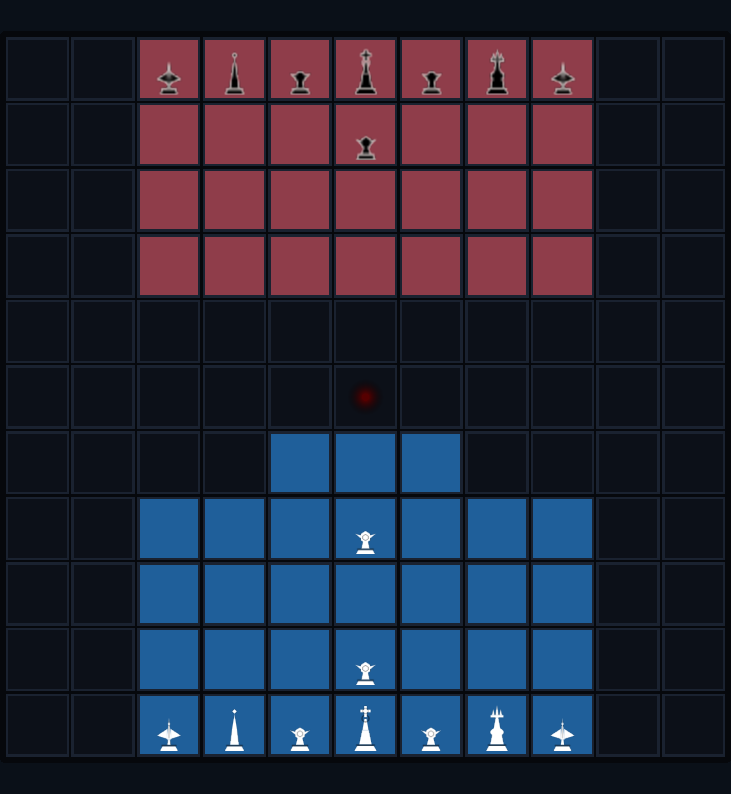
\includegraphics[width=0.55\textwidth]{figures/missions/mission-ai-fleet-skirmish/ply-000}\\
{\small\textbf{Starting position.}}
\end{center}
\clearpage
\plyfig{figures/missions/mission-ai-fleet-skirmish/ply-001}{Ply 1 --- White Infiltrator (8,0)$\rightarrow$(6,3)}{White Infiltrator to (6,3).\; {\color{gray}\scriptsize [net 31--28]}}%
\hfill
\plyfig{figures/missions/mission-ai-fleet-skirmish/ply-002}{Ply 2 --- Black Infiltrator (2,10)$\rightarrow$(1,2)}{Black Infiltrator to (1,2).\; {\color{gray}\scriptsize [net 31--28]}}%

\vspace{0.9em}

\plyfig{figures/missions/mission-ai-fleet-skirmish/ply-003}{Ply 3 --- White Infiltrator (2,0)$\rightarrow$(1,2)}{White takes an early infiltrator at (1,2) to loosen the screen.\; {\color{gray}\scriptsize [captures Infiltrator \,\textbullet\, net 31--28]}}%
\hfill
\plyfig{figures/missions/mission-ai-fleet-skirmish/ply-004}{Ply 4 --- Black Infiltrator (8,10)$\rightarrow$(1,2)}{Black takes an early infiltrator at (1,2) to loosen the screen.\; {\color{gray}\scriptsize [captures Infiltrator \,\textbullet\, net 31--28]}}%

\vspace{0.9em}

\clearpage
\plyfig{figures/missions/mission-ai-fleet-skirmish/ply-005}{Ply 5 --- White Infiltrator (6,3)$\rightarrow$(1,2)}{White takes an early infiltrator at (1,2) to loosen the screen.\; {\color{gray}\scriptsize [captures Infiltrator \,\textbullet\, net 31--28]}}%
\hfill
\plyfig{figures/missions/mission-ai-fleet-skirmish/ply-006}{Ply 6 --- Black Command Hub (5,10)$\rightarrow$(6,9)}{Black Command Hub to (6,9).\; {\color{gray}\scriptsize [net 31--35]}}%

\vspace{0.9em}

\plyfig{figures/missions/mission-ai-fleet-skirmish/ply-007}{Ply 7 --- White Infiltrator (1,2)$\rightarrow$(2,2)}{White Infiltrator to (2,2).\; {\color{gray}\scriptsize [net 31--35]}}%
\hfill
\plyfig{figures/missions/mission-ai-fleet-skirmish/ply-008}{Ply 8 --- Black Escort (5,9)$\rightarrow$(5,10)}{Black Escort to (5,10).\; {\color{gray}\scriptsize [net 31--35]}}%

\vspace{0.9em}

\clearpage
\plyfig{figures/missions/mission-ai-fleet-skirmish/ply-009}{Ply 9 --- White Infiltrator (2,2)$\rightarrow$(1,2)}{White Infiltrator to (1,2).\; {\color{gray}\scriptsize [net 31--35]}}%
\hfill
\plyfig{figures/missions/mission-ai-fleet-skirmish/ply-010}{Ply 10 --- Black Carrier (7,10)$\rightarrow$(9,8)}{Black Carrier to (9,8).\; {\color{gray}\scriptsize [net 31--35]}}%

\vspace{0.9em}

\plyfig{figures/missions/mission-ai-fleet-skirmish/ply-011}{Ply 11 --- White Carrier (7,0)$\rightarrow$(5,2)}{White Carrier to (5,2).\; {\color{gray}\scriptsize [net 31--35]}}%
\hfill
\plyfig{figures/missions/mission-ai-fleet-skirmish/ply-012}{Ply 12 --- Black Command Hub (6,9)$\rightarrow$(6,8)}{Black Command Hub to (6,8).\; {\color{gray}\scriptsize [net 31--42]}}%

\vspace{0.9em}

\clearpage
\plyfig{figures/missions/mission-ai-fleet-skirmish/ply-013}{Ply 13 --- White Infiltrator (1,2)$\rightarrow$(7,0)}{White Infiltrator to (7,0).\; {\color{gray}\scriptsize [net 31--42]}}%
\hfill
\plyfig{figures/missions/mission-ai-fleet-skirmish/ply-014}{Ply 14 --- Black Escort (6,10)$\rightarrow$(7,10)}{Black Escort to (7,10).\; {\color{gray}\scriptsize [net 31--42]}}%

\vspace{0.9em}

\plyfig{figures/missions/mission-ai-fleet-skirmish/ply-015}{Ply 15 --- White Carrier (5,2)$\rightarrow$(4,1)}{White Carrier to (4,1).\; {\color{gray}\scriptsize [net 31--42]}}%
\hfill
\plyfig{figures/missions/mission-ai-fleet-skirmish/ply-016}{Ply 16 --- Black Refractor (3,10)$\rightarrow$(5,8)}{Black Refractor to (5,8).\; {\color{gray}\scriptsize [net 31--42]}}%

\vspace{0.9em}

\clearpage
\plyfig{figures/missions/mission-ai-fleet-skirmish/ply-017}{Ply 17 --- White Infiltrator (7,0)$\rightarrow$(10,5)}{White Infiltrator to (10,5).\; {\color{gray}\scriptsize [net 31--42]}}%
\hfill
\plyfig{figures/missions/mission-ai-fleet-skirmish/ply-018}{Ply 18 --- Black Command Hub (6,8)$\rightarrow$(7,7)}{Black Command Hub to (7,7).\; {\color{gray}\scriptsize [net 31--51 \,\textbullet\, 1 ship locked]}}%

\vspace{0.9em}

\plyfig{figures/missions/mission-ai-fleet-skirmish/ply-019}{Ply 19 --- White Escort (5,3)$\rightarrow$(5,2)}{White Escort to (5,2).\; {\color{gray}\scriptsize [net 28--51 \,\textbullet\, 1 ship locked]}}%
\hfill
\plyfig{figures/missions/mission-ai-fleet-skirmish/ply-020}{Ply 20 --- Black Command Hub (7,7)$\rightarrow$(6,6)}{Black Command Hub to (6,6).\; {\color{gray}\scriptsize [net 28--55]}}%

\vspace{0.9em}

\clearpage
\plyfig{figures/missions/mission-ai-fleet-skirmish/ply-021}{Ply 21 --- White Infiltrator (10,5)$\rightarrow$(0,0)}{White Infiltrator to (0,0).\; {\color{gray}\scriptsize [net 28--55]}}%
\hfill
\plyfig{figures/missions/mission-ai-fleet-skirmish/ply-022}{Ply 22 --- Black Command Hub (6,6)$\rightarrow$(5,7)}{Black Command Hub to (5,7).\; {\color{gray}\scriptsize [net 28--49]}}%

\vspace{0.9em}

\plyfig{figures/missions/mission-ai-fleet-skirmish/ply-023}{Ply 23 --- White Infiltrator (0,0)$\rightarrow$(9,8)}{White takes at (9,8) with an Infiltrator.\; {\color{gray}\scriptsize [captures Carrier \,\textbullet\, net 28--49]}}%
\hfill
\plyfig{figures/missions/mission-ai-fleet-skirmish/ply-024}{Ply 24 --- Black Command Hub (5,7)$\rightarrow$(4,8)}{Black Command Hub to (4,8).\; {\color{gray}\scriptsize [net 28--44]}}%

\vspace{0.9em}

\clearpage
\plyfig{figures/missions/mission-ai-fleet-skirmish/ply-025}{Ply 25 --- White Infiltrator (9,8)$\rightarrow$(7,3)}{White Infiltrator to (7,3).\; {\color{gray}\scriptsize [net 28--44]}}%
\hfill
\plyfig{figures/missions/mission-ai-fleet-skirmish/ply-026}{Ply 26 --- Black Command Hub (4,8)$\rightarrow$(4,7)}{Black Command Hub to (4,7).\; {\color{gray}\scriptsize [net 28--51]}}%

\vspace{0.9em}

\plyfig{figures/missions/mission-ai-fleet-skirmish/ply-027}{Ply 27 --- White Infiltrator (7,3)$\rightarrow$(2,0)}{White Infiltrator to (2,0).\; {\color{gray}\scriptsize [net 28--51]}}%
\hfill
\plyfig{figures/missions/mission-ai-fleet-skirmish/ply-028}{Ply 28 --- Black Escort (7,10)$\rightarrow$(7,9)}{Black Escort to (7,9).\; {\color{gray}\scriptsize [net 28--52]}}%

\vspace{0.9em}

\clearpage
\plyfig{figures/missions/mission-ai-fleet-skirmish/ply-029}{Ply 29 --- White Carrier (4,1)$\rightarrow$(3,1)}{White Carrier to (3,1).\; {\color{gray}\scriptsize [net 28--52]}}%
\hfill
\plyfig{figures/missions/mission-ai-fleet-skirmish/ply-030}{Ply 30 --- Black Command Hub (4,7)$\rightarrow$(5,7)}{Black Command Hub to (5,7).\; {\color{gray}\scriptsize [net 28--49]}}%

\vspace{0.9em}

\plyfig{figures/missions/mission-ai-fleet-skirmish/ply-031}{Ply 31 --- White Infiltrator (2,0)$\rightarrow$(9,0)}{White Infiltrator to (9,0).\; {\color{gray}\scriptsize [net 28--49]}}%
\hfill
\plyfig{figures/missions/mission-ai-fleet-skirmish/ply-032}{Ply 32 --- Black Escort (4,10)$\rightarrow$(3,10)}{Black Escort to (3,10).\; {\color{gray}\scriptsize [net 28--49]}}%

\vspace{0.9em}

\clearpage
\plyfig{figures/missions/mission-ai-fleet-skirmish/ply-033}{Ply 33 --- White Infiltrator (9,0)$\rightarrow$(9,5)}{White Infiltrator to (9,5).\; {\color{gray}\scriptsize [net 28--49]}}%
\hfill
\plyfig{figures/missions/mission-ai-fleet-skirmish/ply-034}{Ply 34 --- Black Command Hub (5,7)$\rightarrow$(5,6)}{Black Command Hub to (5,6).\; {\color{gray}\scriptsize [net 28--56]}}%

\vspace{0.9em}

\plyfig{figures/missions/mission-ai-fleet-skirmish/ply-035}{Ply 35 --- White Infiltrator (9,5)$\rightarrow$(10,3)}{White Infiltrator to (10,3).\; {\color{gray}\scriptsize [net 28--56]}}%
\hfill
\plyfig{figures/missions/mission-ai-fleet-skirmish/ply-036}{Ply 36 --- Black Refractor (5,8)$\rightarrow$(6,9)}{Black Refractor to (6,9).\; {\color{gray}\scriptsize [net 28--49]}}%

\vspace{0.9em}

\clearpage
\plyfig{figures/missions/mission-ai-fleet-skirmish/ply-037}{Ply 37 --- White Infiltrator (10,3)$\rightarrow$(5,10)}{White removes a defender at (5,10). Late captures usually open the Hub or collapse a relay.\; {\color{gray}\scriptsize [captures Escort \,\textbullet\, net 28--49]}}%
\hfill
\plyfig{figures/missions/mission-ai-fleet-skirmish/ply-038}{Ply 38 --- Black Escort (3,10)$\rightarrow$(2,10)}{Black Escort to (2,10).\; {\color{gray}\scriptsize [net 28--49]}}%

\vspace{0.9em}

\plyfig{figures/missions/mission-ai-fleet-skirmish/ply-039}{Ply 39 --- White Infiltrator (5,10)$\rightarrow$(2,10)}{White removes a defender at (2,10). Late captures usually open the Hub or collapse a relay.\; {\color{gray}\scriptsize [captures Escort \,\textbullet\, net 28--49]}}%
\hfill
\plyfig{figures/missions/mission-ai-fleet-skirmish/ply-040}{Ply 40 --- Black Command Hub (5,6)$\rightarrow$(5,7)}{Black Command Hub to (5,7).\; {\color{gray}\scriptsize [net 28--49 \,\textbullet\, 1 ship locked]}}%

\vspace{0.9em}

\clearpage

\vspace{1em}
\noindent\textbf{Debrief.} Same Sensor Net law as Standard Beams --- wider geometry from the Heavy wing. Scan files and diagonals; refuse hangs on both.
\clearpage
\section{AI Mission --- Infiltrator deep dive (49 plies)}
Heuristic AI vs Heuristic AI on hybrid-fleet. Warps through unclaimed space, then a Target-Locked crawl that kills the folding-drive.

\begin{center}

\includegraphics[width=0.55\textwidth]{figures/missions/mission-ai-infiltrator/ply-000}\\
{\small\textbf{Starting position.}}
\end{center}
\clearpage
\plyfig{figures/missions/mission-ai-infiltrator/ply-001}{Ply 1 --- White Infiltrator (3,0)$\rightarrow$(9,10)}{White Infiltrator to (9,10).\; {\color{gray}\scriptsize [net 31--28]}}%
\hfill
\plyfig{figures/missions/mission-ai-infiltrator/ply-002}{Ply 2 --- Black Infiltrator (3,10)$\rightarrow$(9,10)}{Black takes an early infiltrator at (9,10) to loosen the screen.\; {\color{gray}\scriptsize [captures Infiltrator \,\textbullet\, net 31--28]}}%

\vspace{0.9em}

\plyfig{figures/missions/mission-ai-infiltrator/ply-003}{Ply 3 --- White Infiltrator (7,0)$\rightarrow$(9,10)}{White takes an early infiltrator at (9,10) to loosen the screen.\; {\color{gray}\scriptsize [captures Infiltrator \,\textbullet\, net 31--28]}}%
\hfill
\plyfig{figures/missions/mission-ai-infiltrator/ply-004}{Ply 4 --- Black Infiltrator (7,10)$\rightarrow$(9,10)}{Black takes an early infiltrator at (9,10) to loosen the screen.\; {\color{gray}\scriptsize [captures Infiltrator \,\textbullet\, net 31--28]}}%

\vspace{0.9em}

\clearpage
\plyfig{figures/missions/mission-ai-infiltrator/ply-005}{Ply 5 --- White Beam (2,0)$\rightarrow$(2,3)}{White Beam to (2,3).\; {\color{gray}\scriptsize [net 31--28]}}%
\hfill
\plyfig{figures/missions/mission-ai-infiltrator/ply-006}{Ply 6 --- Black Infiltrator (9,10)$\rightarrow$(9,0)}{Black Infiltrator to (9,0).\; {\color{gray}\scriptsize [net 31--28]}}%

\vspace{0.9em}

\plyfig{figures/missions/mission-ai-infiltrator/ply-007}{Ply 7 --- White Beam (8,0)$\rightarrow$(8,3)}{White Beam to (8,3).\; {\color{gray}\scriptsize [net 31--28]}}%
\hfill
\plyfig{figures/missions/mission-ai-infiltrator/ply-008}{Ply 8 --- Black Beam (8,10)$\rightarrow$(8,7)}{Black Beam to (8,7).\; {\color{gray}\scriptsize [net 31--28]}}%

\vspace{0.9em}

\clearpage
\plyfig{figures/missions/mission-ai-infiltrator/ply-009}{Ply 9 --- White Beam (2,3)$\rightarrow$(4,3)}{White Beam to (4,3).\; {\color{gray}\scriptsize [net 31--28]}}%
\hfill
\plyfig{figures/missions/mission-ai-infiltrator/ply-010}{Ply 10 --- Black Beam (2,10)$\rightarrow$(2,7)}{Black Beam to (2,7).\; {\color{gray}\scriptsize [net 31--28]}}%

\vspace{0.9em}

\plyfig{figures/missions/mission-ai-infiltrator/ply-011}{Ply 11 --- White Beam (8,3)$\rightarrow$(6,3)}{White Beam to (6,3).\; {\color{gray}\scriptsize [net 31--28]}}%
\hfill
\plyfig{figures/missions/mission-ai-infiltrator/ply-012}{Ply 12 --- Black Beam (8,7)$\rightarrow$(5,7)}{Black Beam to (5,7).\; {\color{gray}\scriptsize [net 31--28]}}%

\vspace{0.9em}

\clearpage
\plyfig{figures/missions/mission-ai-infiltrator/ply-013}{Ply 13 --- White Escort (5,3)$\rightarrow$(5,4)}{White Escort to (5,4).\; {\color{gray}\scriptsize [net 34--28]}}%
\hfill
\plyfig{figures/missions/mission-ai-infiltrator/ply-014}{Ply 14 --- Black Beam (2,7)$\rightarrow$(4,7)}{Black Beam to (4,7).\; {\color{gray}\scriptsize [net 34--28]}}%

\vspace{0.9em}

\plyfig{figures/missions/mission-ai-infiltrator/ply-015}{Ply 15 --- White Beam (6,3)$\rightarrow$(6,5)}{White Beam to (6,5).\; {\color{gray}\scriptsize [net 34--28]}}%
\hfill
\plyfig{figures/missions/mission-ai-infiltrator/ply-016}{Ply 16 --- Black Escort (6,10)$\rightarrow$(6,9)}{Black Escort to (6,9).\; {\color{gray}\scriptsize [net 34--28]}}%

\vspace{0.9em}

\clearpage
\plyfig{figures/missions/mission-ai-infiltrator/ply-017}{Ply 17 --- White Beam (4,3)$\rightarrow$(4,5)}{White Beam to (4,5).\; {\color{gray}\scriptsize [net 28--28]}}%
\hfill
\plyfig{figures/missions/mission-ai-infiltrator/ply-018}{Ply 18 --- Black Infiltrator (9,0)$\rightarrow$(4,5)}{Black takes at (4,5) with an Infiltrator.\; {\color{gray}\scriptsize [captures Beam \,\textbullet\, net 28--28]}}%

\vspace{0.9em}

\plyfig{figures/missions/mission-ai-infiltrator/ply-019}{Ply 19 --- White Escort (4,0)$\rightarrow$(4,1)}{White Escort to (4,1).\; {\color{gray}\scriptsize [net 28--28]}}%
\hfill
\plyfig{figures/missions/mission-ai-infiltrator/ply-020}{Ply 20 --- Black Infiltrator (4,5)$\rightarrow$(6,5)}{Black takes at (6,5) with an Infiltrator.\; {\color{gray}\scriptsize [captures Beam \,\textbullet\, net 28--28]}}%

\vspace{0.9em}

\clearpage
\plyfig{figures/missions/mission-ai-infiltrator/ply-021}{Ply 21 --- White Escort (4,1)$\rightarrow$(4,2)}{White Escort to (4,2).\; {\color{gray}\scriptsize [net 34--28 \,\textbullet\, 1 ship locked]}}%
\hfill
\plyfig{figures/missions/mission-ai-infiltrator/ply-022}{Ply 22 --- Black Escort (6,9)$\rightarrow$(6,8)}{Black Escort to (6,8).\; {\color{gray}\scriptsize [net 34--28 \,\textbullet\, 1 ship locked]}}%

\vspace{0.9em}

\plyfig{figures/missions/mission-ai-infiltrator/ply-023}{Ply 23 --- White Escort (6,0)$\rightarrow$(6,1)}{White Escort to (6,1).\; {\color{gray}\scriptsize [net 34--28 \,\textbullet\, 1 ship locked]}}%
\hfill
\plyfig{figures/missions/mission-ai-infiltrator/ply-024}{Ply 24 --- Black Escort (6,8)$\rightarrow$(6,7)}{Black Escort to (6,7).\; {\color{gray}\scriptsize [net 34--31 \,\textbullet\, 1 ship locked]}}%

\vspace{0.9em}

\clearpage
\plyfig{figures/missions/mission-ai-infiltrator/ply-025}{Ply 25 --- White Escort (5,1)$\rightarrow$(5,2)}{White Escort to (5,2).\; {\color{gray}\scriptsize [net 34--31 \,\textbullet\, 1 ship locked]}}%
\hfill
\plyfig{figures/missions/mission-ai-infiltrator/ply-026}{Ply 26 --- Black Escort (6,7)$\rightarrow$(6,6)}{Black Escort to (6,6).\; {\color{gray}\scriptsize [net 34--34 \,\textbullet\, 1 ship locked]}}%

\vspace{0.9em}

\plyfig{figures/missions/mission-ai-infiltrator/ply-027}{Ply 27 --- White Escort (4,2)$\rightarrow$(4,3)}{White Escort to (4,3).\; {\color{gray}\scriptsize [net 35--34 \,\textbullet\, 1 ship locked]}}%
\hfill
\plyfig{figures/missions/mission-ai-infiltrator/ply-028}{Ply 28 --- Black Beam (5,7)$\rightarrow$(5,6)}{Black Beam to (5,6).\; {\color{gray}\scriptsize [net 35--34 \,\textbullet\, 1 ship locked]}}%

\vspace{0.9em}

\clearpage
\plyfig{figures/missions/mission-ai-infiltrator/ply-029}{Ply 29 --- White Command Hub (5,0)$\rightarrow$(5,1)}{White Command Hub to (5,1).\; {\color{gray}\scriptsize [net 38--34 \,\textbullet\, 1 ship locked]}}%
\hfill
\plyfig{figures/missions/mission-ai-infiltrator/ply-030}{Ply 30 --- Black Escort (5,9)$\rightarrow$(5,8)}{Black Escort to (5,8).\; {\color{gray}\scriptsize [net 38--34 \,\textbullet\, 1 ship locked]}}%

\vspace{0.9em}

\plyfig{figures/missions/mission-ai-infiltrator/ply-031}{Ply 31 --- White Escort (5,2)$\rightarrow$(5,3)}{White Escort to (5,3).\; {\color{gray}\scriptsize [net 38--34 \,\textbullet\, 1 ship locked]}}%
\hfill
\plyfig{figures/missions/mission-ai-infiltrator/ply-032}{Ply 32 --- Black Escort (5,8)$\rightarrow$(5,7)}{Black Escort to (5,7).\; {\color{gray}\scriptsize [net 38--28 \,\textbullet\, 1 ship locked]}}%

\vspace{0.9em}

\clearpage
\plyfig{figures/missions/mission-ai-infiltrator/ply-033}{Ply 33 --- White Escort (4,3)$\rightarrow$(4,4)}{White Escort to (4,4).\; {\color{gray}\scriptsize [net 39--28 \,\textbullet\, 1 ship locked]}}%
\hfill
\plyfig{figures/missions/mission-ai-infiltrator/ply-034}{Ply 34 --- Black Escort (4,10)$\rightarrow$(4,9)}{Black Escort to (4,9).\; {\color{gray}\scriptsize [net 39--35 \,\textbullet\, 1 ship locked]}}%

\vspace{0.9em}

\plyfig{figures/missions/mission-ai-infiltrator/ply-035}{Ply 35 --- White Command Hub (5,1)$\rightarrow$(5,2)}{White Command Hub to (5,2).\; {\color{gray}\scriptsize [net 42--35 \,\textbullet\, 1 ship locked]}}%
\hfill
\plyfig{figures/missions/mission-ai-infiltrator/ply-036}{Ply 36 --- Black Escort (4,9)$\rightarrow$(4,8)}{Black Escort to (4,8).\; {\color{gray}\scriptsize [net 42--35 \,\textbullet\, 1 ship locked]}}%

\vspace{0.9em}

\clearpage
\plyfig{figures/missions/mission-ai-infiltrator/ply-037}{Ply 37 --- White Escort (4,4)$\rightarrow$(4,5)}{White Escort to (4,5).\; {\color{gray}\scriptsize [net 45--35 \,\textbullet\, 2 ships locked]}}%
\hfill
\plyfig{figures/missions/mission-ai-infiltrator/ply-038}{Ply 38 --- Black Beam (4,7)$\rightarrow$(4,6)}{Black Beam to (4,6).\; {\color{gray}\scriptsize [net 45--35 \,\textbullet\, 3 ships locked]}}%

\vspace{0.9em}

\plyfig{figures/missions/mission-ai-infiltrator/ply-039}{Ply 39 --- White Escort (4,5)$\rightarrow$(4,6)}{White takes at (4,6) with an Escort.\; {\color{gray}\scriptsize [captures Beam \,\textbullet\, net 48--35 \,\textbullet\, 4 ships locked]}}%
\hfill
\plyfig{figures/missions/mission-ai-infiltrator/ply-040}{Ply 40 --- Black Beam (5,6)$\rightarrow$(4,6)}{Black takes at (4,6) with a Beam.\; {\color{gray}\scriptsize [captures Escort \,\textbullet\, net 42--35 \,\textbullet\, 1 ship locked]}}%

\vspace{0.9em}

\clearpage
\plyfig{figures/missions/mission-ai-infiltrator/ply-041}{Ply 41 --- White Escort (6,1)$\rightarrow$(6,2)}{White Escort to (6,2).\; {\color{gray}\scriptsize [net 42--35 \,\textbullet\, 1 ship locked]}}%
\hfill
\plyfig{figures/missions/mission-ai-infiltrator/ply-042}{Ply 42 --- Black Command Hub (5,10)$\rightarrow$(5,9)}{Black Command Hub to (5,9).\; {\color{gray}\scriptsize [net 42--38 \,\textbullet\, 1 ship locked]}}%

\vspace{0.9em}

\plyfig{figures/missions/mission-ai-infiltrator/ply-043}{Ply 43 --- White Escort (6,2)$\rightarrow$(6,3)}{White Escort to (6,3).\; {\color{gray}\scriptsize [net 42--38 \,\textbullet\, 1 ship locked]}}%
\hfill
\plyfig{figures/missions/mission-ai-infiltrator/ply-044}{Ply 44 --- Black Escort (5,7)$\rightarrow$(5,6)}{Black Escort to (5,6).\; {\color{gray}\scriptsize [net 42--39 \,\textbullet\, 1 ship locked]}}%

\vspace{0.9em}

\clearpage
\plyfig{figures/missions/mission-ai-infiltrator/ply-045}{Ply 45 --- White Escort (6,3)$\rightarrow$(6,4)}{White Escort to (6,4).\; {\color{gray}\scriptsize [net 42--39 \,\textbullet\, 1 ship locked]}}%
\hfill
\plyfig{figures/missions/mission-ai-infiltrator/ply-046}{Ply 46 --- Black Infiltrator (6,5)$\rightarrow$(6,4)}{Black removes a defender at (6,4). Late captures usually open the Hub or collapse a relay.\; {\color{gray}\scriptsize [captures Escort \,\textbullet\, net 42--39 \,\textbullet\, 1 ship locked]}}%

\vspace{0.9em}

\plyfig{figures/missions/mission-ai-infiltrator/ply-047}{Ply 47 --- White Escort (5,4)$\rightarrow$(6,4)}{White removes a defender at (6,4). Late captures usually open the Hub or collapse a relay.\; {\color{gray}\scriptsize [captures Infiltrator \,\textbullet\, net 42--39]}}%
\hfill
\plyfig{figures/missions/mission-ai-infiltrator/ply-048}{Ply 48 --- Black Command Hub (5,9)$\rightarrow$(5,8)}{Black Command Hub to (5,8).\; {\color{gray}\scriptsize [net 42--42]}}%

\vspace{0.9em}

\clearpage
\plyfig{figures/missions/mission-ai-infiltrator/ply-049}{Ply 49 --- White Escort (6,4)$\rightarrow$(6,5)}{White Escort to (6,5).\; {\color{gray}\scriptsize [net 45--42 \,\textbullet\, 3 ships locked]}}%

\vspace{0.9em}


\vspace{1em}
\noindent\textbf{Debrief.} Phase Runners only warp while undetected. Push into hostile coverage and the engines lock --- one orthogonal step, no jump.
\clearpage
\section{AI Mission --- Lockout squeeze (100 plies)}
Mobility-pressure AI vs Random with the sector clock deferred. Historical near-Lockout teaching window (pre-EMP); immobility is defeat.

\begin{center}

\includegraphics[width=0.55\textwidth]{figures/missions/mission-ai-lockout/ply-000}\\
{\small\textbf{Starting position.}}
\end{center}
\clearpage
\plyfig{figures/missions/mission-ai-lockout/ply-001}{Ply 1 --- White Command Hub (5,0)$\rightarrow$(6,1)}{White Command Hub to (6,1).\; {\color{gray}\scriptsize [net 35--28]}}%
\hfill
\plyfig{figures/missions/mission-ai-lockout/ply-002}{Ply 2 --- Black Infiltrator (3,10)$\rightarrow$(0,9)}{Black Infiltrator to (0,9).\; {\color{gray}\scriptsize [net 35--28]}}%

\vspace{0.9em}

\plyfig{figures/missions/mission-ai-lockout/ply-003}{Ply 3 --- White Infiltrator (3,0)$\rightarrow$(0,9)}{White takes an early infiltrator at (0,9) to loosen the screen.\; {\color{gray}\scriptsize [captures Infiltrator \,\textbullet\, net 35--28]}}%
\hfill
\plyfig{figures/missions/mission-ai-lockout/ply-004}{Ply 4 --- Black Infiltrator (7,10)$\rightarrow$(7,5)}{Black Infiltrator to (7,5).\; {\color{gray}\scriptsize [net 35--28]}}%

\vspace{0.9em}

\clearpage
\plyfig{figures/missions/mission-ai-lockout/ply-005}{Ply 5 --- White Infiltrator (0,9)$\rightarrow$(7,5)}{White takes an early infiltrator at (7,5) to loosen the screen.\; {\color{gray}\scriptsize [captures Infiltrator \,\textbullet\, net 35--28]}}%
\hfill
\plyfig{figures/missions/mission-ai-lockout/ply-006}{Ply 6 --- Black Beam (8,10)$\rightarrow$(8,7)}{Black Beam to (8,7).\; {\color{gray}\scriptsize [net 35--28]}}%

\vspace{0.9em}

\plyfig{figures/missions/mission-ai-lockout/ply-007}{Ply 7 --- White Infiltrator (7,5)$\rightarrow$(0,0)}{White Infiltrator to (0,0).\; {\color{gray}\scriptsize [net 35--28]}}%
\hfill
\plyfig{figures/missions/mission-ai-lockout/ply-008}{Ply 8 --- Black Beam (8,7)$\rightarrow$(8,10)}{Black Beam to (8,10).\; {\color{gray}\scriptsize [net 35--28]}}%

\vspace{0.9em}

\clearpage
\plyfig{figures/missions/mission-ai-lockout/ply-009}{Ply 9 --- White Escort (4,0)$\rightarrow$(3,0)}{White Escort to (3,0).\; {\color{gray}\scriptsize [net 37--28]}}%
\hfill
\plyfig{figures/missions/mission-ai-lockout/ply-010}{Ply 10 --- Black Escort (6,10)$\rightarrow$(7,10)}{Black Escort to (7,10).\; {\color{gray}\scriptsize [net 37--28]}}%

\vspace{0.9em}

\plyfig{figures/missions/mission-ai-lockout/ply-011}{Ply 11 --- White Escort (3,0)$\rightarrow$(4,0)}{White Escort to (4,0).\; {\color{gray}\scriptsize [net 35--28]}}%
\hfill
\plyfig{figures/missions/mission-ai-lockout/ply-012}{Ply 12 --- Black Beam (8,10)$\rightarrow$(8,7)}{Black Beam to (8,7).\; {\color{gray}\scriptsize [net 35--28]}}%

\vspace{0.9em}

\clearpage
\plyfig{figures/missions/mission-ai-lockout/ply-013}{Ply 13 --- White Escort (5,1)$\rightarrow$(4,1)}{White Escort to (4,1).\; {\color{gray}\scriptsize [net 35--28]}}%
\hfill
\plyfig{figures/missions/mission-ai-lockout/ply-014}{Ply 14 --- Black Command Hub (5,10)$\rightarrow$(4,9)}{Black Command Hub to (4,9).\; {\color{gray}\scriptsize [net 35--37]}}%

\vspace{0.9em}

\plyfig{figures/missions/mission-ai-lockout/ply-015}{Ply 15 --- White Infiltrator (0,0)$\rightarrow$(8,7)}{White takes at (8,7) with an Infiltrator.\; {\color{gray}\scriptsize [captures Beam \,\textbullet\, net 35--37]}}%
\hfill
\plyfig{figures/missions/mission-ai-lockout/ply-016}{Ply 16 --- Black Escort (7,10)$\rightarrow$(6,10)}{Black Escort to (6,10).\; {\color{gray}\scriptsize [net 35--35]}}%

\vspace{0.9em}

\clearpage
\plyfig{figures/missions/mission-ai-lockout/ply-017}{Ply 17 --- White Infiltrator (8,7)$\rightarrow$(0,0)}{White Infiltrator to (0,0).\; {\color{gray}\scriptsize [net 35--35]}}%
\hfill
\plyfig{figures/missions/mission-ai-lockout/ply-018}{Ply 18 --- Black Escort (4,10)$\rightarrow$(3,10)}{Black Escort to (3,10).\; {\color{gray}\scriptsize [net 35--35]}}%

\vspace{0.9em}

\plyfig{figures/missions/mission-ai-lockout/ply-019}{Ply 19 --- White Infiltrator (0,0)$\rightarrow$(0,2)}{White Infiltrator to (0,2).\; {\color{gray}\scriptsize [net 35--35]}}%
\hfill
\plyfig{figures/missions/mission-ai-lockout/ply-020}{Ply 20 --- Black Escort (5,9)$\rightarrow$(6,9)}{Black Escort to (6,9).\; {\color{gray}\scriptsize [net 35--35]}}%

\vspace{0.9em}

\clearpage
\plyfig{figures/missions/mission-ai-lockout/ply-021}{Ply 21 --- White Infiltrator (0,2)$\rightarrow$(0,0)}{White Infiltrator to (0,0).\; {\color{gray}\scriptsize [net 35--35]}}%
\hfill
\plyfig{figures/missions/mission-ai-lockout/ply-022}{Ply 22 --- Black Command Hub (4,9)$\rightarrow$(4,10)}{Black Command Hub to (4,10).\; {\color{gray}\scriptsize [net 35--28]}}%

\vspace{0.9em}

\plyfig{figures/missions/mission-ai-lockout/ply-023}{Ply 23 --- White Command Hub (6,1)$\rightarrow$(5,2)}{White Command Hub to (5,2).\; {\color{gray}\scriptsize [net 42--28]}}%
\hfill
\plyfig{figures/missions/mission-ai-lockout/ply-024}{Ply 24 --- Black Escort (3,10)$\rightarrow$(3,9)}{Black Escort to (3,9).\; {\color{gray}\scriptsize [net 42--28]}}%

\vspace{0.9em}

\clearpage
\plyfig{figures/missions/mission-ai-lockout/ply-025}{Ply 25 --- White Command Hub (5,2)$\rightarrow$(6,1)}{White Command Hub to (6,1).\; {\color{gray}\scriptsize [net 35--28]}}%
\hfill
\plyfig{figures/missions/mission-ai-lockout/ply-026}{Ply 26 --- Black Beam (2,10)$\rightarrow$(2,9)}{Black Beam to (2,9).\; {\color{gray}\scriptsize [net 35--28]}}%

\vspace{0.9em}

\plyfig{figures/missions/mission-ai-lockout/ply-027}{Ply 27 --- White Command Hub (6,1)$\rightarrow$(7,2)}{White Command Hub to (7,2).\; {\color{gray}\scriptsize [net 45--28]}}%
\hfill
\plyfig{figures/missions/mission-ai-lockout/ply-028}{Ply 28 --- Black Escort (6,10)$\rightarrow$(5,10)}{Black Escort to (5,10).\; {\color{gray}\scriptsize [net 45--28]}}%

\vspace{0.9em}

\clearpage
\plyfig{figures/missions/mission-ai-lockout/ply-029}{Ply 29 --- White Escort (4,1)$\rightarrow$(4,2)}{White Escort to (4,2).\; {\color{gray}\scriptsize [net 46--28]}}%
\hfill
\plyfig{figures/missions/mission-ai-lockout/ply-030}{Ply 30 --- Black Escort (3,9)$\rightarrow$(4,9)}{Black Escort to (4,9).\; {\color{gray}\scriptsize [net 46--28]}}%

\vspace{0.9em}

\plyfig{figures/missions/mission-ai-lockout/ply-031}{Ply 31 --- White Escort (4,2)$\rightarrow$(3,2)}{White Escort to (3,2).\; {\color{gray}\scriptsize [net 49--28]}}%
\hfill
\plyfig{figures/missions/mission-ai-lockout/ply-032}{Ply 32 --- Black Escort (5,10)$\rightarrow$(5,9)}{Black Escort to (5,9).\; {\color{gray}\scriptsize [net 49--28]}}%

\vspace{0.9em}

\clearpage
\plyfig{figures/missions/mission-ai-lockout/ply-033}{Ply 33 --- White Escort (4,0)$\rightarrow$(4,1)}{White Escort to (4,1).\; {\color{gray}\scriptsize [net 49--28]}}%
\hfill
\plyfig{figures/missions/mission-ai-lockout/ply-034}{Ply 34 --- Black Escort (4,9)$\rightarrow$(4,8)}{Black Escort to (4,8).\; {\color{gray}\scriptsize [net 49--28]}}%

\vspace{0.9em}

\plyfig{figures/missions/mission-ai-lockout/ply-035}{Ply 35 --- White Escort (6,0)$\rightarrow$(5,0)}{White Escort to (5,0).\; {\color{gray}\scriptsize [net 49--28]}}%
\hfill
\plyfig{figures/missions/mission-ai-lockout/ply-036}{Ply 36 --- Black Escort (6,9)$\rightarrow$(7,9)}{Black Escort to (7,9).\; {\color{gray}\scriptsize [net 49--31]}}%

\vspace{0.9em}

\clearpage
\plyfig{figures/missions/mission-ai-lockout/ply-037}{Ply 37 --- White Escort (5,0)$\rightarrow$(4,0)}{White Escort to (4,0).\; {\color{gray}\scriptsize [net 49--31]}}%
\hfill
\plyfig{figures/missions/mission-ai-lockout/ply-038}{Ply 38 --- Black Escort (4,8)$\rightarrow$(4,9)}{Black Escort to (4,9).\; {\color{gray}\scriptsize [net 49--31]}}%

\vspace{0.9em}

\plyfig{figures/missions/mission-ai-lockout/ply-039}{Ply 39 --- White Command Hub (7,2)$\rightarrow$(6,2)}{White Command Hub to (6,2).\; {\color{gray}\scriptsize [net 45--31]}}%
\hfill
\plyfig{figures/missions/mission-ai-lockout/ply-040}{Ply 40 --- Black Escort (5,9)$\rightarrow$(5,10)}{Black Escort to (5,10).\; {\color{gray}\scriptsize [net 45--31]}}%

\vspace{0.9em}

\clearpage
\plyfig{figures/missions/mission-ai-lockout/ply-041}{Ply 41 --- White Command Hub (6,2)$\rightarrow$(7,3)}{White Command Hub to (7,3).\; {\color{gray}\scriptsize [net 56--31]}}%
\hfill
\plyfig{figures/missions/mission-ai-lockout/ply-042}{Ply 42 --- Black Escort (4,9)$\rightarrow$(5,9)}{Black Escort to (5,9).\; {\color{gray}\scriptsize [net 56--31]}}%

\vspace{0.9em}

\plyfig{figures/missions/mission-ai-lockout/ply-043}{Ply 43 --- White Escort (4,0)$\rightarrow$(5,0)}{White Escort to (5,0).\; {\color{gray}\scriptsize [net 56--31]}}%
\hfill
\plyfig{figures/missions/mission-ai-lockout/ply-044}{Ply 44 --- Black Beam (2,9)$\rightarrow$(2,8)}{Black Beam to (2,8).\; {\color{gray}\scriptsize [net 56--31]}}%

\vspace{0.9em}

\clearpage
\plyfig{figures/missions/mission-ai-lockout/ply-045}{Ply 45 --- White Command Hub (7,3)$\rightarrow$(6,3)}{White Command Hub to (6,3).\; {\color{gray}\scriptsize [net 52--31]}}%
\hfill
\plyfig{figures/missions/mission-ai-lockout/ply-046}{Ply 46 --- Black Beam (2,8)$\rightarrow$(2,9)}{Black Beam to (2,9).\; {\color{gray}\scriptsize [net 52--31]}}%

\vspace{0.9em}

\plyfig{figures/missions/mission-ai-lockout/ply-047}{Ply 47 --- White Escort (4,1)$\rightarrow$(4,0)}{White Escort to (4,0).\; {\color{gray}\scriptsize [net 52--31]}}%
\hfill
\plyfig{figures/missions/mission-ai-lockout/ply-048}{Ply 48 --- Black Beam (2,9)$\rightarrow$(3,9)}{Black Beam to (3,9).\; {\color{gray}\scriptsize [net 52--31]}}%

\vspace{0.9em}

\clearpage
\plyfig{figures/missions/mission-ai-lockout/ply-049}{Ply 49 --- White Escort (5,0)$\rightarrow$(5,1)}{White Escort to (5,1).\; {\color{gray}\scriptsize [net 52--31]}}%
\hfill
\plyfig{figures/missions/mission-ai-lockout/ply-050}{Ply 50 --- Black Beam (3,9)$\rightarrow$(3,10)}{Black Beam to (3,10).\; {\color{gray}\scriptsize [net 52--31]}}%

\vspace{0.9em}

\plyfig{figures/missions/mission-ai-lockout/ply-051}{Ply 51 --- White Command Hub (6,3)$\rightarrow$(7,3)}{White Command Hub to (7,3).\; {\color{gray}\scriptsize [net 56--31]}}%
\hfill
\plyfig{figures/missions/mission-ai-lockout/ply-052}{Ply 52 --- Black Command Hub (4,10)$\rightarrow$(3,9)}{Black Command Hub to (3,9).\; {\color{gray}\scriptsize [net 56--41]}}%

\vspace{0.9em}

\clearpage
\plyfig{figures/missions/mission-ai-lockout/ply-053}{Ply 53 --- White Escort (4,0)$\rightarrow$(3,0)}{White Escort to (3,0).\; {\color{gray}\scriptsize [net 57--41]}}%
\hfill
\plyfig{figures/missions/mission-ai-lockout/ply-054}{Ply 54 --- Black Command Hub (3,9)$\rightarrow$(2,8)}{Black Command Hub to (2,8).\; {\color{gray}\scriptsize [net 57--45]}}%

\vspace{0.9em}

\plyfig{figures/missions/mission-ai-lockout/ply-055}{Ply 55 --- White Escort (3,0)$\rightarrow$(4,0)}{White Escort to (4,0).\; {\color{gray}\scriptsize [net 56--45]}}%
\hfill
\plyfig{figures/missions/mission-ai-lockout/ply-056}{Ply 56 --- Black Escort (7,9)$\rightarrow$(7,10)}{Black Escort to (7,10).\; {\color{gray}\scriptsize [net 56--43]}}%

\vspace{0.9em}

\clearpage
\plyfig{figures/missions/mission-ai-lockout/ply-057}{Ply 57 --- White Command Hub (7,3)$\rightarrow$(6,2)}{White Command Hub to (6,2).\; {\color{gray}\scriptsize [net 45--43]}}%
\hfill
\plyfig{figures/missions/mission-ai-lockout/ply-058}{Ply 58 --- Black Beam (3,10)$\rightarrow$(2,10)}{Black Beam to (2,10).\; {\color{gray}\scriptsize [net 45--36]}}%

\vspace{0.9em}

\plyfig{figures/missions/mission-ai-lockout/ply-059}{Ply 59 --- White Infiltrator (7,0)$\rightarrow$(7,10)}{White takes at (7,10) with an Infiltrator.\; {\color{gray}\scriptsize [captures Escort \,\textbullet\, net 45--36]}}%
\hfill
\plyfig{figures/missions/mission-ai-lockout/ply-060}{Ply 60 --- Black Command Hub (2,8)$\rightarrow$(3,7)}{Black Command Hub to (3,7).\; {\color{gray}\scriptsize [net 45--49]}}%

\vspace{0.9em}

\clearpage
\plyfig{figures/missions/mission-ai-lockout/ply-061}{Ply 61 --- White Escort (4,0)$\rightarrow$(4,1)}{White Escort to (4,1).\; {\color{gray}\scriptsize [net 45--49]}}%
\hfill
\plyfig{figures/missions/mission-ai-lockout/ply-062}{Ply 62 --- Black Command Hub (3,7)$\rightarrow$(4,8)}{Black Command Hub to (4,8).\; {\color{gray}\scriptsize [net 45--42 \,\textbullet\, 1 ship locked]}}%

\vspace{0.9em}

\plyfig{figures/missions/mission-ai-lockout/ply-063}{Ply 63 --- White Command Hub (6,2)$\rightarrow$(7,2)}{White Command Hub to (7,2).\; {\color{gray}\scriptsize [net 49--42 \,\textbullet\, 1 ship locked]}}%
\hfill
\plyfig{figures/missions/mission-ai-lockout/ply-064}{Ply 64 --- Black Command Hub (4,8)$\rightarrow$(3,8)}{Black Command Hub to (3,8).\; {\color{gray}\scriptsize [net 49--42]}}%

\vspace{0.9em}

\clearpage
\plyfig{figures/missions/mission-ai-lockout/ply-065}{Ply 65 --- White Command Hub (7,2)$\rightarrow$(6,2)}{White Command Hub to (6,2).\; {\color{gray}\scriptsize [net 45--42]}}%
\hfill
\plyfig{figures/missions/mission-ai-lockout/ply-066}{Ply 66 --- Black Beam (2,10)$\rightarrow$(2,8)}{Black Beam to (2,8).\; {\color{gray}\scriptsize [net 45--42]}}%

\vspace{0.9em}

\plyfig{figures/missions/mission-ai-lockout/ply-067}{Ply 67 --- White Command Hub (6,2)$\rightarrow$(5,2)}{White Command Hub to (5,2).\; {\color{gray}\scriptsize [net 42--42]}}%
\hfill
\plyfig{figures/missions/mission-ai-lockout/ply-068}{Ply 68 --- Black Command Hub (3,8)$\rightarrow$(3,7)}{Black Command Hub to (3,7).\; {\color{gray}\scriptsize [net 42--49]}}%

\vspace{0.9em}

\clearpage
\plyfig{figures/missions/mission-ai-lockout/ply-069}{Ply 69 --- White Command Hub (5,2)$\rightarrow$(6,2)}{White Command Hub to (6,2).\; {\color{gray}\scriptsize [net 45--49]}}%
\hfill
\plyfig{figures/missions/mission-ai-lockout/ply-070}{Ply 70 --- Black Beam (2,8)$\rightarrow$(2,10)}{Black Beam to (2,10).\; {\color{gray}\scriptsize [net 45--49]}}%

\vspace{0.9em}

\plyfig{figures/missions/mission-ai-lockout/ply-071}{Ply 71 --- White Escort (4,1)$\rightarrow$(4,2)}{White Escort to (4,2).\; {\color{gray}\scriptsize [net 45--49]}}%
\hfill
\plyfig{figures/missions/mission-ai-lockout/ply-072}{Ply 72 --- Black Escort (5,10)$\rightarrow$(6,10)}{Black Escort to (6,10).\; {\color{gray}\scriptsize [net 45--51 \,\textbullet\, 1 ship locked]}}%

\vspace{0.9em}

\clearpage
\plyfig{figures/missions/mission-ai-lockout/ply-073}{Ply 73 --- White Infiltrator (7,10)$\rightarrow$(6,10)}{White takes at (6,10) with an Infiltrator.\; {\color{gray}\scriptsize [captures Escort \,\textbullet\, net 45--49 \,\textbullet\, 1 ship locked]}}%
\hfill
\plyfig{figures/missions/mission-ai-lockout/ply-074}{Ply 74 --- Black Command Hub (3,7)$\rightarrow$(3,6)}{Black Command Hub to (3,6).\; {\color{gray}\scriptsize [net 45--49 \,\textbullet\, 1 ship locked]}}%

\vspace{0.9em}

\plyfig{figures/missions/mission-ai-lockout/ply-075}{Ply 75 --- White Infiltrator (0,0)$\rightarrow$(2,10)}{White takes at (2,10) with an Infiltrator.\; {\color{gray}\scriptsize [captures Beam \,\textbullet\, net 45--49 \,\textbullet\, 1 ship locked]}}%
\hfill
\plyfig{figures/missions/mission-ai-lockout/ply-076}{Ply 76 --- Black Escort (5,9)$\rightarrow$(5,8)}{Black Escort to (5,8).\; {\color{gray}\scriptsize [net 45--49 \,\textbullet\, 1 ship locked]}}%

\vspace{0.9em}

\clearpage
\plyfig{figures/missions/mission-ai-lockout/ply-077}{Ply 77 --- White Command Hub (6,2)$\rightarrow$(6,3)}{White Command Hub to (6,3).\; {\color{gray}\scriptsize [net 52--49 \,\textbullet\, 3 ships locked]}}%
\hfill
\plyfig{figures/missions/mission-ai-lockout/ply-078}{Ply 78 --- Black Command Hub (3,6)$\rightarrow$(2,6)}{Black Command Hub to (2,6).\; {\color{gray}\scriptsize [net 52--42 \,\textbullet\, 1 ship locked]}}%

\vspace{0.9em}

\plyfig{figures/missions/mission-ai-lockout/ply-079}{Ply 79 --- White Command Hub (6,3)$\rightarrow$(5,4)}{White Command Hub to (5,4).\; {\color{gray}\scriptsize [net 52--42 \,\textbullet\, 3 ships locked]}}%
\hfill
\plyfig{figures/missions/mission-ai-lockout/ply-080}{Ply 80 --- Black Command Hub (2,6)$\rightarrow$(1,6)}{Black Command Hub to (1,6).\; {\color{gray}\scriptsize [net 52--35]}}%

\vspace{0.9em}

\clearpage
\plyfig{figures/missions/mission-ai-lockout/ply-081}{Ply 81 --- White Infiltrator (2,10)$\rightarrow$(5,8)}{White takes at (5,8) with an Infiltrator.\; {\color{gray}\scriptsize [captures Escort \,\textbullet\, net 52--35]}}%
\hfill
\plyfig{figures/missions/mission-ai-lockout/ply-082}{Ply 82 --- Black Command Hub (1,6)$\rightarrow$(0,7)}{Black Command Hub to (0,7).\; {\color{gray}\scriptsize [net 52--28]}}%

\vspace{0.9em}

\plyfig{figures/missions/mission-ai-lockout/ply-083}{Ply 83 --- White Escort (3,2)$\rightarrow$(2,2)}{White Escort to (2,2).\; {\color{gray}\scriptsize [net 55--28]}}%
\hfill
\plyfig{figures/missions/mission-ai-lockout/ply-084}{Ply 84 --- Black Command Hub (0,7)$\rightarrow$(0,6)}{Black Command Hub to (0,6).\; {\color{gray}\scriptsize [net 55--28]}}%

\vspace{0.9em}

\clearpage
\plyfig{figures/missions/mission-ai-lockout/ply-085}{Ply 85 --- White Command Hub (5,4)$\rightarrow$(6,4)}{White Command Hub to (6,4).\; {\color{gray}\scriptsize [net 58--28]}}%
\hfill
\plyfig{figures/missions/mission-ai-lockout/ply-086}{Ply 86 --- Black Command Hub (0,6)$\rightarrow$(1,5)}{Black Command Hub to (1,5).\; {\color{gray}\scriptsize [net 58--35 \,\textbullet\, 2 ships locked]}}%

\vspace{0.9em}

\plyfig{figures/missions/mission-ai-lockout/ply-087}{Ply 87 --- White Command Hub (6,4)$\rightarrow$(5,4)}{White Command Hub to (5,4).\; {\color{gray}\scriptsize [net 55--35 \,\textbullet\, 2 ships locked]}}%
\hfill
\plyfig{figures/missions/mission-ai-lockout/ply-088}{Ply 88 --- Black Command Hub (1,5)$\rightarrow$(1,6)}{Black Command Hub to (1,6).\; {\color{gray}\scriptsize [net 55--35]}}%

\vspace{0.9em}

\clearpage
\plyfig{figures/missions/mission-ai-lockout/ply-089}{Ply 89 --- White Command Hub (5,4)$\rightarrow$(4,3)}{White Command Hub to (4,3).\; {\color{gray}\scriptsize [net 49--35 \,\textbullet\, 2 ships locked]}}%
\hfill
\plyfig{figures/missions/mission-ai-lockout/ply-090}{Ply 90 --- Black Command Hub (1,6)$\rightarrow$(1,7)}{Black Command Hub to (1,7).\; {\color{gray}\scriptsize [net 49--35]}}%

\vspace{0.9em}

\plyfig{figures/missions/mission-ai-lockout/ply-091}{Ply 91 --- White Command Hub (4,3)$\rightarrow$(4,4)}{White Command Hub to (4,4).\; {\color{gray}\scriptsize [net 52--35 \,\textbullet\, 2 ships locked]}}%
\hfill
\plyfig{figures/missions/mission-ai-lockout/ply-092}{Ply 92 --- Black Command Hub (1,7)$\rightarrow$(0,7)}{Black Command Hub to (0,7).\; {\color{gray}\scriptsize [net 52--28]}}%

\vspace{0.9em}

\clearpage
\plyfig{figures/missions/mission-ai-lockout/ply-093}{Ply 93 --- White Command Hub (4,4)$\rightarrow$(3,4)}{White Command Hub to (3,4).\; {\color{gray}\scriptsize [net 52--28 \,\textbullet\, 2 ships locked]}}%
\hfill
\plyfig{figures/missions/mission-ai-lockout/ply-094}{Ply 94 --- Black Command Hub (0,7)$\rightarrow$(0,8)}{Black Command Hub to (0,8).\; {\color{gray}\scriptsize [net 52--24]}}%

\vspace{0.9em}

\plyfig{figures/missions/mission-ai-lockout/ply-095}{Ply 95 --- White Command Hub (3,4)$\rightarrow$(2,5)}{White Command Hub to (2,5).\; {\color{gray}\scriptsize [net 42--24 \,\textbullet\, 2 ships locked]}}%
\hfill
\plyfig{figures/missions/mission-ai-lockout/ply-096}{Ply 96 --- Black Command Hub (0,8)$\rightarrow$(0,7)}{Black Command Hub to (0,7).\; {\color{gray}\scriptsize [net 42--28 \,\textbullet\, 2 ships locked]}}%

\vspace{0.9em}

\clearpage
\plyfig{figures/missions/mission-ai-lockout/ply-097}{Ply 97 --- White Escort (5,1)$\rightarrow$(5,0)}{White Escort to (5,0).\; {\color{gray}\scriptsize [net 42--28 \,\textbullet\, 2 ships locked]}}%
\hfill
\plyfig{figures/missions/mission-ai-lockout/ply-098}{Ply 98 --- Black Command Hub (0,7)$\rightarrow$(1,7)}{Black Command Hub to (1,7).\; {\color{gray}\scriptsize [net 42--35 \,\textbullet\, 2 ships locked]}}%

\vspace{0.9em}

\plyfig{figures/missions/mission-ai-lockout/ply-099}{Ply 99 --- White Command Hub (2,5)$\rightarrow$(3,5)}{White Command Hub to (3,5).\; {\color{gray}\scriptsize [net 58--35 \,\textbullet\, 2 ships locked]}}%
\hfill
\plyfig{figures/missions/mission-ai-lockout/ply-100}{Ply 100 --- Black Command Hub (1,7)$\rightarrow$(2,7)}{Black Command Hub to (2,7).\; {\color{gray}\scriptsize [net 58--42 \,\textbullet\, 3 ships locked]}}%

\vspace{0.9em}

\clearpage

\vspace{1em}
\noindent\textbf{Debrief.} Bodies alone rarely reach true zero replies while a Hub lives. See Mission 4 for Command Overload finishing Lockout.
\clearpage

\end{document}
